\documentclass[compress]{beamer}
\usetheme{Warsaw}
\useoutertheme{split}

%%%%%%%%%%%%%%%%%%%%%%%%%%%%%%%%%%%%%%%%%%%%%%%%%%%%%%%%%%%%%%%
% Improvement on the default split theme : added line numbers %
%%%%%%%%%%%%%%%%%%%%%%%%%%%%%%%%%%%%%%%%%%%%%%%%%%%%%%%%%%%%%%%

%%%%%%%%%%%%%%%
% Main colors %
%%%%%%%%%%%%%%%

\setbeamercolor{frametitle}{fg=white}
\setbeamercolor{frametitle right}{fg=white}
\setbeamercolor{structure}{fg=beamer@blendedblue} % this should be the default anyway, but make sure, since we change it between basic/advanced slides
\setbeamercolor{goodpractice head}{fg=white,bg=orange!85!black}
\setbeamercolor{goodpractice body}{fg=black,bg=orange!25}

%%%%%%%%%%%%%%%%%%%%%%%%%
% headline and footline %
%%%%%%%%%%%%%%%%%%%%%%%%%

\defbeamertemplate*{footline}{mysplit theme}
{%
  \leavevmode%
  \hbox{\begin{beamercolorbox}[wd=.5\paperwidth,ht=2.5ex,dp=1.125ex,leftskip=.3cm plus1fill,rightskip=.3cm]{author in head/foot}%
    \usebeamerfont{author in head/foot}\insertshortauthor%
  \end{beamercolorbox}%
  \begin{beamercolorbox}[wd=.4\paperwidth,ht=2.5ex,dp=1.125ex,leftskip=.3cm,rightskip=.3cm plus1fil]{title in head/foot}%
    \usebeamerfont{title in head/foot}\insertshorttitle%
  \end{beamercolorbox}}%
    \begin{beamercolorbox}[wd=.1\paperwidth,ht=2.5ex,dp=1.125ex,leftskip=.1cm plus1fill,rightskip=.1cm]{date in head/foot}%
      \usebeamerfont{date in head/foot} \insertframenumber{} / \inserttotalframenumber%
    \end{beamercolorbox}%
  \vskip0pt%
}

\defbeamertemplate*{headline}{mysplit theme}
{%
  \leavevmode%
  \begin{beamercolorbox}[wd=.4\paperwidth,ht=2.5ex,dp=1.125ex]{section in head/foot}%
    \insertsectionnavigationhorizontal{.4\paperwidth}{\hskip0pt plus1filll}{}%
  \end{beamercolorbox}%
  \begin{beamercolorbox}[wd=.6\paperwidth,ht=2.5ex,dp=1.125ex]{subsection in head/foot}%
    \insertsubsectionnavigationhorizontal{.6\paperwidth}{}{\hskip0pt plus1filll}%
  \end{beamercolorbox}%
}

%%%%%%%%%%%%
% packages %
%%%%%%%%%%%%

\usepackage{morewrites}
\usepackage[utf8]{inputenc}
\usepackage{newunicodechar}
\usepackage{scontents}
\makeatletter
\let\verbatimsc\@undefined
\let\endverbatimsc\@undefined
\makeatother
\usepackage{minted}
\newminted{tex}{linenos}
\newenvironment{verbatimsc}
               {\VerbatimEnvironment
                 \begin{minted}[linenos,escapeinside=||]{cpp}}
               {\end{minted}}
\newcommand\highlightCppCode[2]{
  \renewenvironment{verbatimsc}
                   {\VerbatimEnvironment
                     \begin{minted}[linenos,highlightlines={#1},escapeinside=||]{cpp}}
                   {\end{minted}}
  \typestored{#2}
}
\newminted{cpp}{gobble=4,linenos}
\newminted{shell-session}{gobble=4}
\newminted[makefile]{shell-session}{gobble=4}
\newminted{python}{linenos=true,gobble=4}
\newmintinline[cppinline]{cpp}{}

\usepackage{fancyvrb}
\newcommand*{\fvtextcolor}[2]{\textcolor{#1}{#2}}

\usepackage{pgf}
\usepackage{pgffor}
\usepackage{tikz}
\usetikzlibrary{arrows,arrows.meta,automata,positioning,snakes,shapes}

\usepackage{tcolorbox}

\usepackage[framemethod=TikZ]{mdframed}
\mdfdefinestyle{simplebox}{roundcorner=4pt,linewidth=0,backgroundcolor=blue!50!black,fontcolor=white}

\usepackage{multicol}
\usepackage{tikz-uml}

\usepackage{booktabs}
\usepackage{comment}
\usepackage{totcount}
\usepackage{xspace}

% Use C++Course.cut for output so it's cleaned by latexmk
\def\DefaultCutFileName{\def\CommentCutFile{\jobname.cut}}
\DefaultCutFileName

%%%%%%%%%%%%%%%%%%%
% useful commands %
%%%%%%%%%%%%%%%%%%%
\newcommand{\cpp}{C$^{++}$\xspace}
\newcommand{\deprecated}{\textcolor{red}{\bf Deprecated}}
\newcommand{\removed}{\textcolor{red}{\bf Removed}}


%%%%%%%%%%%%%%%%%%%%%%%%%%%%%%%%%%%%%%%%%%%%%%%%%
% boxes with good practices                     %
% Use \begin{goodpractice}{Title} to create one %
%%%%%%%%%%%%%%%%%%%%%%%%%%%%%%%%%%%%%%%%%%%%%%%%%
\makeatletter
\newcommand\listofgoodpractices{%
  \addtocontents{lgp}{\end{enumerate}}
  \scriptsize
  \begin{multicols}{2}
    \@starttoc{lgp}%
  \end{multicols}
}
\AtBeginDocument{ \addtocontents{lgp}{\begin{enumerate} } }

\newcounter{gp@counter}
\def\gp@lasttitle{None}

\newenvironment{goodpracticeWithShortcut}[2]
{%
  % Generate an entry in the index of good practices. In case of slide overlays, we only generate
  % an entry for the first slide of the overlay set by saving the last title of the
  % good practice box.
  \ifthenelse{\equal{\gp@lasttitle}{#1}}{}{%
    \hypertarget<1>{goodpractice.\thegp@counter}{}
    \addtocontents{lgp}{\protect\item \protect\hyperlink{goodpractice.\thegp@counter}{#2\protect\hfill\insertframenumber}}
    \stepcounter{gp@counter}
    \gdef\gp@lasttitle{#1}
  }
  % The box that shows up on the slide
  \begin{beamerboxesrounded}[upper=goodpractice head,lower=goodpractice body,shadow=true]{Good practice: #1}
}%
{%
  \end{beamerboxesrounded}
}
\newenvironment{goodpractice}[2][]
{%
  \ifthenelse{\equal{#1}{}}%
    { \begin{goodpracticeWithShortcut}{#2}{#2} }
    { \begin{goodpracticeWithShortcut}{#2}{#1} }
}%
{%
  \end{goodpracticeWithShortcut}
}

%%%%%%%%%%%%%%%%%%%%%%%%%%%%%%%%%%%%%%%%%%%%%%%%%
% boxes with exercises                          %
% Use \begin{exercise}{Title} to create one     %
%%%%%%%%%%%%%%%%%%%%%%%%%%%%%%%%%%%%%%%%%%%%%%%%%
\newcommand\listofexercises{%
  \addtocontents{lex}{\end{enumerate}}
  \scriptsize
  \begin{multicols}{3}
    \@starttoc{lex}%
  \end{multicols}
}
\AtBeginDocument{ \addtocontents{lex}{\begin{enumerate} } }

\newcounter{ex@counter}
\regtotcounter{ex@counter}

\newenvironment{exerciseWithShortcut}[2]
{%
  \hypertarget<1>{exercise.\theex@counter}{}
  \addtocontents{lex}{\protect\item \protect\hyperlink{exercise.\theex@counter}{#2\protect\hfill\insertframenumber}}
  \stepcounter{ex@counter}
  % The box that shows up on the slide
  \begin{alertblock}{Exercise: #1}
}%
{%
  \end{alertblock}
}
\newenvironment{exercise}[1]
{%
  \begin{exerciseWithShortcut}{#1}{#1}
}%
{%
  \end{exerciseWithShortcut}
}

%%%%%%%%%%%%%%%%%%%%%%%%%%%%%%%
% frametitle with C++ version %
%%%%%%%%%%%%%%%%%%%%%%%%%%%%%%%
% Use as \frametitlecpp[14]{Title}
\newcommand\frametitlecpp[2][98]{
  \frametitle{#2 \hfill \cpp#1}
}

%%%%%%%%%%%%%%%%%%%%%%%%%%%%%%%%%%%%%%%%
% easy links to godbolt and cppinsight %
%%%%%%%%%%%%%%%%%%%%%%%%%%%%%%%%%%%%%%%%
\newcommand\listofgodbolt{%
  \addtocontents{lgb}{\end{enumerate}}
  \scriptsize
  \begin{multicols}{2}
    \@starttoc{lgb}%
  \end{multicols}
}
\AtBeginDocument{ \addtocontents{lgb}{\begin{enumerate} } }

\newcounter{gb@counter}
\regtotcounter{gb@counter}
\resetcounteronoverlays{gb@counter}
\newcommand*{\overlaynumber}{\number\beamer@slideinframe}

% Use as \godboltLink{url}
\newcommand\godboltLink[2]{%
  \href{#1}{\color{blue!50!white} godbolt}%
  \ifnum \overlaynumber=1%
    \hypertarget<1>{godbolt.\thegb@counter}{}
    \addtocontents{lgb}{\protect\item \protect\hyperlink{godbolt.\thegb@counter}{#2 - \href{#1}{godbolt}\protect\hfill\insertframenumber}}%
    \stepcounter{gb@counter}%
  \fi
}

% Use as \begin{exampleblockGB}{<Title of box on slide>}{<godbolt link>}{<title in index>}
\newenvironment{exampleblockGB}[3]
{%
  \begin{exampleblock}{#1 - \godboltLink{#2}{#3}}
}%
{%
  \end{exampleblock}
}

% Use as \cppinsightLink{url}
\newcommand\cppinsightLink[1]{%
  \href{#1}{\color{blue!50!white} cppinsight}%
}
% Use as \cppinsightLink{url}
\newcommand\cpprefLink[1]{%
  \href{#1}{\color{blue!50!white} cppreference}%
}

% Use as \youtubechannel{channelname}
\newcommand\youtubechannel[1]{%
  \mbox{\href{https://www.youtube.com/c/#1}{\color{red!10!black}\raisebox{-0.1em}{\includegraphics[height=0.8em]{youtube}}\ #1}}%
}

% Use as \youtubeuser{username}
\newcommand\youtubeuser[1]{%
  \mbox{\href{https://www.youtube.com/user/#1}{\color{red!10!black}\raisebox{-0.1em}{\includegraphics[height=0.8em]{youtube}}\ #1}}%
}

\makeatother

%%%%%%%%%%%%%%%%%%%%%%%%%%%%%%%
% easy class diagrams in tikz %
%%%%%%%%%%%%%%%%%%%%%%%%%%%%%%%

\newcommand\classbox[3][]{
  \def\temp{#3}
  \ifx\temp\empty
    \draw[thick] node (#2) [#1]
         [rectangle,rounded corners,draw] {#2};
  \else
    \draw[thick] node (#2) [#1]
         [rectangle,rounded corners,draw] {
      \begin{tabular}{l}
        \multicolumn{1}{c}{#2} \\
        \hline
        #3
      \end{tabular}
    };
  \fi
}

%%%%%%%%%%%%%%%%%%%%%%%%%%%%%%%%%%%%%%
% easy memory stack diagrams in tikz %
%%%%%%%%%%%%%%%%%%%%%%%%%%%%%%%%%%%%%%

\newcounter{memorystackindex}

\pgfkeys{
  memorystack/.is family,
  memorystack,
  size x/.initial=4cm,
  size y/.initial=.5cm,
  word size/.initial=4,
  block size/.initial=1,
  nb blocks/.initial=8,
  base address/.initial=12288,
  color/.initial=black,
  addresses/.initial=1
}

\makeatletter

\newcommand\memorystackset[1]{\pgfkeys{memorystack,#1}}
\newcommand\memorystack[1][]{
  \memorystackset{#1,
    size x/.get=\stacksizex,
    size y/.get=\stacksizey,
    word size/.get=\stackwordsize,
    block size/.get=\blocksize,
    nb blocks/.get=\stacknbblocks,
    base address/.get=\stackbaseaddr,
    color/.get=\stackcolor,
    addresses/.get=\displayaddrs
  }
  \draw[thick,\stackcolor,text=white] node (title)
        at (\stacksizex/2, \stacknbblocks*\stacksizey+.5cm)
        [rectangle,rounded corners,fill=blue!50!black] {Memory layout};
  \setcounter{memorystackindex}{1}
  \draw[thick,\stackcolor] (0,0) rectangle (\stacksizex,\stacknbblocks*\stacksizey);
  \pgfmathsetmacro{\nbbars}{\stacknbblocks-1}
  \pgfmathtruncatemacro\nbbarstrunc{\nbbars}
  \ifnum\nbbarstrunc>0
    \foreach \n in {1,...,\nbbarstrunc} {
      \draw[\stackcolor!70] (0,\n*\stacksizey) -- +(\stacksizex,0);
    }
  \fi
  \foreach \n in {1,...,\stacknbblocks} {
    \foreach \p in {1,...,\stackwordsize} {
      \draw node (stack\n-\p)
            at (\stacksizex/\stackwordsize*\p-\stacksizex/\stackwordsize/2,\n*\stacksizey-\stacksizey/2)
            [rectangle,minimum width=\stacksizex,minimum height=\stacksizey] {};
    }
    \ifnum1=\displayaddrs\relax
      \pgfmathparse{(\n-1)*\blocksize*\stackwordsize+\stackbaseaddr}
      \pgfmathtruncatemacro\addressdec{\pgfmathresult}
      \pgfmathdectoBase\hexversion{\addressdec}{16}
      \draw node at (\stacksizex,\n*\stacksizey-\stacksizey/2) [right=2pt]
            {0x\hexversion};
    \fi
  }
  \pgfmathsetmacro{\nbseps}{\stackwordsize-1}
  \pgfmathtruncatemacro\nbsepstrunc{\nbseps}
  \ifnum\nbsepstrunc>0
    \foreach \n in {1,...,\nbsepstrunc} {
      \draw[\stackcolor!10] (\stacksizex/\stackwordsize*\n,0) -- +(0,\stacknbblocks*\stacksizey);
    }
  \fi
}

\newcommand\memorypushvalue[3]{
  \draw node at (stack#1-#2) {#3};
}

\newcommand\memorypushwidevalue[1]{
  \memorystackset{
    size x/.get=\stacksizex,
    size y/.get=\stacksizey,
  }
  \draw node (content) at (\stacksizex/2,\value{memorystackindex}*\stacksizey-\stacksizey/2) {#1};
  \draw[\stackcolor!80,->] (content) -- (.2cm,\value{memorystackindex}*\stacksizey-\stacksizey/2);
  \draw[\stackcolor!80,->] (content) -- (\stacksizex-.2cm,\value{memorystackindex}*\stacksizey-\stacksizey/2);
  \addtocounter{memorystackindex}{1}
}

\newcommand\memorypushhalfvalue[1]{
  \memorystackset{
    size x/.get=\stacksizex,
    size y/.get=\stacksizey,
  }
  \draw node (content) at (\stacksizex/4,\value{memorystackindex}*\stacksizey-\stacksizey/2) {#1};
  \draw[\stackcolor!80,->] (content) -- (.2cm,\value{memorystackindex}*\stacksizey-\stacksizey/2);
  \draw[\stackcolor!80,->] (content) -- (\stacksizex/2-.2cm,\value{memorystackindex}*\stacksizey-\stacksizey/2);
  \addtocounter{memorystackindex}{1}
}

\newcounter{localcount}
\newcommand\memorypush[1]{
  \memorystackset{
    word size/.get=\stackwordsize,
    nb blocks/.get=\stacknbblocks
  }
  \count@=0
  \setcounter{localcount}{1}
  \@for\v:=#1\do{
    \ifnum\count@<\stackwordsize
      \advance\count@ 1
      \memorypushvalue{\arabic{memorystackindex}}{\arabic{localcount}}{\v}
    \fi
    \addtocounter{localcount}{1}
  }
  \addtocounter{memorystackindex}{1}
}

\newcommand\memorypushpointer[2][]{
  \memorystackset{
    word size/.get=\stackwordsize,
    base address/.get=\stackbaseaddr,
    block size/.get=\blocksize,
  }
  \pgfmathparse{(#2-1)*\stackwordsize*\blocksize+\stackbaseaddr}
  \pgfmathtruncatemacro\addressdec{\pgfmathresult}
  \pgfmathdectoBase\hexaddress{\addressdec}{16}
  \memorypushvalue{\arabic{memorystackindex}}{1}{#1 0x\hexaddress}
  \draw[\stackcolor!80,->] (stack\arabic{memorystackindex}-1.west) .. controls +(left:1) and +(left:1) .. (stack#2-1.west);
  \addtocounter{memorystackindex}{1}
}

\newcommand\memorystruct[3]{
  \memorystackset{
    size y/.get=\stacksizey
  }
  \draw[snake=brace,thick] (-2pt,#1*\stacksizey-\stacksizey) -- (-2pt,#2*\stacksizey)
    node [midway, above, sloped] {#3};
}

\newcommand\memorygoto[1]{
  \setcounter{memorystackindex}{#1}
}
\makeatother

%%%%%%%%%%%%%%%%%%
% Document setup %
%%%%%%%%%%%%%%%%%%

\title{HEP \cpp course}
\author[B. Gruber, S. Hageboeck, S. Ponce]{B. Gruber, S. Hageboeck, S. Ponce \\ \texttt{sebastien.ponce@cern.ch}}
\institute{CERN}
\date{\today}
\pgfdeclareimage[height=0.5cm]{cernlogo}{CERN-logo.jpg}
\logo{\pgfuseimage{cernlogo}}

\AtBeginSection[] {
  \begin{frame}<beamer>
    \frametitle{\insertsection}
    \begin{multicols}{2}
      \tableofcontents[sectionstyle=show/shaded,subsectionstyle=show/show/hide]
    \end{multicols}
  \end{frame}
}

\AtBeginSubsection[] {
  \begin{frame}<beamer>
    \frametitle{\insertsubsection}
    \tableofcontents[sectionstyle=show/hide,subsectionstyle=show/shaded/hide]
  \end{frame}
}

\hypersetup{
  colorlinks=true,
  allcolors=.,
  urlcolor={blue!80!white}
}


% setup for the basic/advanced course switch
% create a new latex if called basic (false by default)
\newif\ifbasic
%\basictrue % uncomment to make basic true
\IfFileExists{onlybasics.tex}{\input{onlybasics}}{}

% create a comment environment advanced. depending on the value of basic, we exclude or include it.
\ifbasic
  \excludecomment{advanced}
\else
  % advanced slides have a different structure color
  \specialcomment{advanced}{
    \setbeamercolor{structure}{fg=beamer@blendedblue!40!violet}
  }{
    \setbeamercolor{structure}{fg=beamer@blendedblue}
  }
\fi

\newunicodechar{σ}{$\sigma$}
\newunicodechar{µ}{$\mu$}

\begin{document}

\showboxdepth=\maxdimen
\showboxbreadth=\maxdimen

\begin{frame}
  \titlepage
\end{frame}

\begin{frame}
  \frametitle{Foreword}
  \begin{block}{What this course is not}
    \begin{itemize}
    \item It is not for absolute beginners
    \item It is not for experts
    \item It is not complete at all (would need 3 weeks...)
      \begin{itemize}
      \item although it is already too long for the time we have
      \item \inserttotalframenumber{} slides, \insertpresentationendpage{} pages, \total{ex@counter} exercises...
      \end{itemize}
    \end{itemize}
  \end{block}
  \begin{block}{How I see it}
    \begin{description}
    \item[Adaptative] pick what you want
    \item[Interactive] tell me what to skip/insist on
    \item[Practical] let's spend time on real code
    \end{description}
  \end{block}
  \begin{block}{Where to find latest version ?}
    \begin{itemize}
    \item full sources at {\scriptsize \url{https://github.com/hsf-training/cpluspluscourse}}
    \item latest pdf under {\scriptsize \href{https://github.com/hsf-training/cpluspluscourse/raw/download/talk/C++Course\_full.pdf}{raw/download/talk/C++Course\_full.pdf}}
    \end{itemize}
  \end{block}
\end{frame}


\begin{frame}
  \frametitle{More courses}
  \begin{block}{The HSF Software Training Center}
    A set of course modules on more software engineering aspects prepared from within the HEP community
    \begin{itemize}
      \item Unix shell
      \item Python
      \item Version control (git, gitlab, github)
      \item ...
    \end{itemize}
    {\small \url{https://hepsoftwarefoundation.org/training/curriculum.html}}
  \end{block}

\end{frame}

\begin{frame}
  \frametitle{Outline}
  \begin{multicols}{2}
    \tableofcontents[sectionstyle=show,subsectionstyle=hide]
  \end{multicols}
\end{frame}

\begin{frame}
  \frametitle{Detailed outline}
  %\vspace{-0.5cm}
  \begin{tiny}
    \begin{multicols}{3}
      \tableofcontents[sectionstyle=show,subsectionstyle=show]
    \end{multicols}
  \end{tiny}
\end{frame}

\section[Intro]{History and goals}
\input{introduction/history}
\input{introduction/goals}

\section[base]{Language basics}
\input{basicconcepts/coresyntax}
\subsection[Ptr]{Arrays and Pointers}

\begin{frame}[fragile]
  \frametitlecpp[98]{Static arrays}
  \begin{cppcode}
    int ai[4] = {1,2,3,4};
    int ai[] = {1,2,3,4};  // identical

    char ac[3] = {'a','b','c'};   // char array
    char ac[4] = "abc";           // valid C string
    char ac[4] = {'a','b','c',0}; // same valid string

    int i = ai[2];  // i = 3
    char c = ac[8]; // at best garbage, may segfault
    int i = ai[4];  // also garbage !
  \end{cppcode}
\end{frame}

\Scontents*[store-cmd=code_arrays]{
int i = 4;
int *pi = &i;
int j = *pi + 1;

int ai[] = {1,2,3};
int *pai = ai; // decay to ptr
int *paj = pai + 1;
int k = *paj + 1;

// compile error
int *pak = k;

// seg fault !
int *pak = (int*)k;
int l = *pak;
}
\begin{frame}[fragile]
  \frametitlecpp[98]{Pointers}
  \begin{multicols}{2}
  \begin{overprint}[\columnwidth]
    \onslide<1> \highlightCppCode{}{code_arrays}
    \onslide<2> \highlightCppCode{1}{code_arrays}
    \onslide<3> \highlightCppCode{2}{code_arrays}
    \onslide<4> \highlightCppCode{3}{code_arrays}
    \onslide<5> \highlightCppCode{5}{code_arrays}
    \onslide<6> \highlightCppCode{6}{code_arrays}
    \onslide<7> \highlightCppCode{7}{code_arrays}
    \onslide<8> \highlightCppCode{8}{code_arrays}
    \onslide<9> \highlightCppCode{11}{code_arrays}
  \end{overprint}
  \columnbreak
    \onslide<2->{
      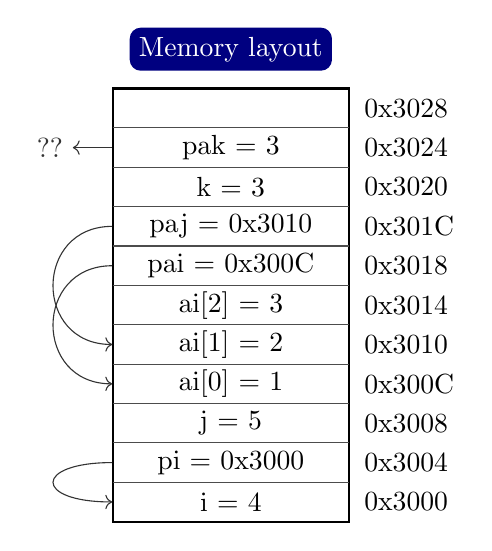
\begin{tikzpicture}
        \memorystack[size x=3cm,word size=1,block size=4,nb blocks=11]
        \onslide<2-> {\memorypush{i = 4}}
        \onslide<3-> {\memorypushpointer[pi =]{1}}
        \onslide<4-> {\memorypush{j = 5}}
        \onslide<5-> {\memorypush{ai[0] = 1}}
        \onslide<5-> {\memorypush{ai[1] = 2}}
        \onslide<5-> {\memorypush{ai[2] = 3}}
        \onslide<6-> {\memorypushpointer[pai =]{4}}
        \onslide<7-> {\memorypushpointer[paj =]{5}}
        \onslide<8-> {\memorypush{k = 3}}
        \onslide<9-> {\memorypush{pak = 3}}
        \onslide<9-> {\draw[\stackcolor!80,->] (stack10-1.west) -- +(-0.5cm,0)
          node [anchor=east] {??};}
      \end{tikzpicture}
    }
  \end{multicols}
\end{frame}

\begin{frame}[fragile]
  \frametitlecpp[11]{nullptr}
  \begin{block}{A pointer to nothing}
    \begin{itemize}
    \item if a pointer doesn't point to anything, set it to \cppinline{nullptr}
    \begin{itemize}
      \item useful to e.g.\ mark the end of a linked data structure
      \item or absence of an optional function argument (pointer)
    \end{itemize}
    \item same as setting it to 0 or \cppinline{NULL} (before \cpp11)
    \item triggers compilation error when assigned to integer
    \end{itemize}
  \end{block}
  \pause
  \begin{exampleblock}{Example code}
    \begin{cppcode*}{}
      int* ip = nullptr;
      int i = NULL;      // compiles, bug?
      int i = nullptr;   // ERROR
    \end{cppcode*}
  \end{exampleblock}
\end{frame}

\begin{frame}[fragile]
  \frametitlecpp[98]{Dynamic arrays using C}
  \begin{cppcode}
    #include <cstdlib>
    #include <cstring>

    int *bad;          // pointer to random address
    int *ai = nullptr; // better, deterministic, testable

    // allocate array of 10 ints (uninitialized)
    ai = (int*) malloc(10*sizeof(int));
    memset(ai, 0, 10*sizeof(int)); // and set them to 0

    ai = (int*) calloc(10, sizeof(int)); // both in one go

    free(ai); // release memory
  \end{cppcode}
  \begin{goodpractice}[C's memory management]{Don't use C's memory management}
    Use \cppinline{std::vector} and friends or smart pointers
  \end{goodpractice}
\end{frame}

\begin{frame}[fragile]
  \frametitlecpp[98]{Manual dynamic arrays using \cpp}
  \begin{cppcode}
    #include <cstdlib>
    #include <cstring>

    // allocate array of 10 ints
    int* ai = new int[10];   // uninitialized
    int* ai = new int[10]{}; // zero-initialized

    delete[] ai; // release array memory

    // allocate a single int
    int* pi = new int;
    int* pi = new int{};
    delete pi; // release scalar memory
  \end{cppcode}
  \begin{goodpractice}[Manual memory management]{Don't use manual memory management}
    Use \cppinline{std::vector} and friends or smart pointers
  \end{goodpractice}
\end{frame}

\input{basicconcepts/scopesnamespaces}
\input{basicconcepts/classenum}
\input{basicconcepts/references}
\input{basicconcepts/functions}
\input{basicconcepts/operators}
\subsection[Control]{Control structures}

\begin{frame}[fragile]
  \frametitlecpp[98]{Control structures: if}
  \begin{block}{if syntax}
    \begin{cppcode*}{}
      if (condition1) {
        Statement1; Statement2;
      } else if (condition2)
        OnlyOneStatement;
      else {
        Statement3;
        Statement4;
      }
    \end{cppcode*}
    \begin{itemize}
      \item The \cppinline{else} and \cppinline{else if} clauses are optional
      \item The \cppinline{else if} clause can be repeated
      \item Braces are optional if there is a single statement
    \end{itemize}
  \end{block}
\end{frame}

\begin{frame}[fragile]
  \frametitlecpp[98]{Control structures: if}
  \begin{exampleblock}{Practical example}
    \begin{cppcode*}{}
      int collatz(int a) {
        if (a <= 0) {
          std::cout << "not supported\n";
          return 0;
        } else if (a == 1) {
          return 1;
        } else if (a%2 == 0) {
          return collatz(a/2);
        } else {
          return collatz(3*a+1);
        }
      }
    \end{cppcode*}
  \end{exampleblock}
\end{frame}

\begin{frame}[fragile]
  \frametitlecpp[98]{Control structures: conditional operator}
  \begin{block}{Syntax}
    \begin{cppcode*}{linenos=false}
      test ? expression1 : expression2;
    \end{cppcode*}
    \vspace{-0.2cm}
    \begin{itemize}
      \item If test is \cppinline{true} \cppinline{expression1} is returned
      \item Else, \cppinline{expression2} is returned
    \end{itemize}
  \end{block}
  \pause
  \begin{exampleblock}{Practical example}
    \begin{cppcode*}{}
      const int charge = isLepton ? -1 : 0;
    \end{cppcode*}
  \end{exampleblock}
  \pause
  \begin{alertblock}{Do not abuse it}
    \begin{cppcode*}{}
      int collatz(int a) {
        return a==1 ? 1 : collatz(a%2==0 ? a/2 : 3*a+1);
      }
    \end{cppcode*}
    \begin{itemize}
      \item Explicit \cppinline{if}s are generally easier to read
      \item Use the ternary operator with short conditions and expressions
      \item Avoid nesting
    \end{itemize}
  \end{alertblock}
\end{frame}

\begin{frame}[fragile]
  \frametitlecpp[98]{Control structures: switch}
  \begin{block}{Syntax}
    \begin{cppcode*}{gobble=0}
      switch(identifier) {
        case c1 : statements1; break;
        case c2 : statements2; break;
        case c3 : statements3; break;
        ...
        default : statementsn; break;
      }
    \end{cppcode*}
    \begin{itemize}
      \item The \cppinline{break} statement is not mandatory but...
      \item Cases are entry points, not independent pieces
      \item Execution ``falls through'' to the next case without a \cppinline{break}!
      \item The \cppinline{default} case may be omitted
    \end{itemize}
  \end{block}
  \pause
  \begin{alertblock}{Use break}
    Avoid \cppinline{switch} statements with fall-through cases
  \end{alertblock}
\end{frame}

\begin{frame}[fragile]
  \frametitlecpp[98]{Control structures: switch}
  \begin{exampleblock}{Practical example}
    \begin{cppcode*}{}
      enum class Lang { French, German, English, Other };
      Lang language = ...;
      switch (language) {
        case Lang::French:
          std::cout << "Bonjour";
          break;
        case Lang::German:
          std::cout << "Guten Tag";
          break;
        case Lang::English:
          std::cout << "Good morning";
          break;
        default:
          std::cout << "I do not speak your language";
      }
    \end{cppcode*}
  \end{exampleblock}
\end{frame}

\AtBeginEnvironment{minted}{\renewcommand{\fcolorbox}[4][]{#4}}

\begin{frame}[fragile]
  \frametitlecpp[17]{\texttt{[[fallthrough]]} attribute}
  \begin{block}{New compiler warning}
    Since \cpp17, compilers are encouraged to warn on fall-through
  \end{block}
  \begin{exampleblock}{\cpp17}
    \begin{cppcode*}{}
      switch (c) {
        case 'a':
          f();    // Warning emitted
        case 'b': // Warning probably suppressed
        case 'c':
          g();
          [[fallthrough]]; // Warning suppressed
        case 'd':
          h();
      }
    \end{cppcode*}
  \end{exampleblock}
\end{frame}

\begin{frame}[fragile]
  \frametitlecpp[17]{Init-statements for if and switch}
  \begin{block}{Purpose}
    Allows to limit variable scope in \cppinline{if} and \cppinline{switch} statements
  \end{block}
  \begin{exampleblock}{\cpp17}
    \begin{cppcode*}{}
      if (Value val = GetValue(); condition(val)) {
        f(val); // ok
      } else
        g(val); // ok
      h(val);   // error, no `val` in scope here
    \end{cppcode*}
  \end{exampleblock}
  \pause
  \begin{alertblock}{\cpp98}
    Don't confuse with a variable declaration as condition:
    \begin{cppcode*}{firstnumber=7}
      if (Value* val = GetValuePtr())
        f(*val);
    \end{cppcode*}
  \end{alertblock}
\end{frame}

\begin{frame}[fragile]
  \frametitlecpp[98]{Control structures: for loop}
  \begin{block}{for loop syntax}
    \begin{cppcode*}{}
      for(initializations; condition; increments) {
        statements;
      }
    \end{cppcode*}
    \vspace{-0.2cm}
    \begin{itemize}
      \item Initializations and increments are comma separated
      \item Initializations can contain declarations
      \item Braces are optional if loop body is a single statement
    \end{itemize}
  \end{block}
  \pause
  \begin{exampleblock}{Practical example}
    \begin{cppcode*}{firstnumber=4}
      for(int i = 0, j = 0 ; i < 10 ; i++, j = i*i) {
        std::cout << i << "^2 is " << j << '\n';
      }
    \end{cppcode*}
  \end{exampleblock}
  \pause
  \begin{goodpractice}[\texttt{for} syntax]{Don't abuse the \texttt{for} syntax}
    \begin{itemize}
      \item The \cppinline{for} loop head should fit in 1-3 lines
    \end{itemize}
  \end{goodpractice}
\end{frame}

\begin{frame}[fragile]
  \frametitlecpp[11]{Range-based loops}
  \begin{block}{Reason of being}
    \begin{itemize}
    \item Simplifies loops over ``ranges'' tremendously
    \item Especially with STL containers and ranges
    \end{itemize}
  \end{block}
  \begin{block}{Syntax}
    \begin{cppcode*}{}
      for ( type iteration_variable : range ) {
        // body using iteration_variable
      }
    \end{cppcode*}
  \end{block}
  \begin{exampleblock}{Example code}
    \begin{cppcode*}{firstnumber=4}
      int v[4] = {1,2,3,4};
      int sum = 0;
      for (int a : v) { sum += a; }
    \end{cppcode*}
  \end{exampleblock}
\end{frame}

\begin{frame}[fragile]
  \frametitlecpp[20]{Init-statements for range-based loops}
  \begin{block}{Purpose}
    Allows to limit variable scope in range-based loops
  \end{block}
  \begin{alertblock}{\cpp17}
    \begin{cppcode*}{}
      std::array data = {"hello", ",", "world"};
      std::size_t i = 0;
      for (auto& d : data) {
        std::cout << i++ << ' ' << d << '\n';
      }
    \end{cppcode*}
  \end{alertblock}
  \begin{exampleblock}{\cpp20}
    \begin{cppcode*}{firstnumber=6}
      for (std::size_t i = 0; auto const & d : data) {
        std::cout << i++ << ' ' << d << '\n';
      }
    \end{cppcode*}
  \end{exampleblock}
\end{frame}

\begin{frame}[fragile]
  \frametitlecpp[98]{Control structures: while loop}
  \begin{block}{while loop syntax}
    \begin{cppcode*}{}
      while(condition) {
        statements;
      }

      do {
        statements;
      } while(condition);
    \end{cppcode*}
    \begin{itemize}
      \item Braces are optional if the body is a single statement
    \end{itemize}
  \end{block}
  \pause
  \begin{alertblock}{Bad example}
    \begin{cppcode*}{}
      while (n != 1)
        if (0 == n%2) n /= 2;
        else n = 3 * n + 1;
    \end{cppcode*}
  \end{alertblock}
\end{frame}

\begin{frame}[fragile]
  \frametitlecpp[98]{Control structures: jump statements}
  \begin{block}{}
    \begin{description}
    \item[break] Exits the loop and continues after it
    \item[continue] Goes immediately to next loop iteration
    \item[return] Exits the current function
    \item[goto] Can jump anywhere inside a function, avoid!
    \end{description}
  \end{block}
  \pause
  \begin{alertblock}{Bad example}
    \begin{cppcode*}{}
      while (1) {
        if (n == 1) break;
        if (0 == n%2) {
          std::cout << n << '\n';
          n /= 2;
          continue;
        }
        n = 3 * n + 1;
      }
    \end{cppcode*}
  \end{alertblock}
\end{frame}

\begin{frame}[fragile]
  \frametitlecpp[11]{Control structures}
  \begin{exerciseWithShortcut}{Control structures}{Control structs}
    Familiarise yourself with different kinds of control structures. Re-implement them in different ways.
    \begin{itemize}
      \item Go to \texttt{exercises/control}
      \item Look at \texttt{control.cpp}
      \item Compile it (\texttt{make}) and run the program (\texttt{./control})
      \item Work on the tasks that you find in \texttt{README.md}
    \end{itemize}
  \end{exerciseWithShortcut}
\end{frame}

\subsection[.h]{Headers and interfaces}

\begin{frame}[fragile]
  \frametitlecpp[98]{Headers and interfaces}
  \begin{block}{Interface}
    Set of declarations defining some functionality
    \begin{itemize}
    \item Put in a so-called ``header file''
    \item The implementation exists somewhere else
    \end{itemize}
  \end{block}
  \begin{block}{Header: hello.hpp}
    \begin{cppcode*}{linenos=false}
      void printHello();
    \end{cppcode*}
  \end{block}
  \begin{block}{Usage: myfile.cpp}
    \begin{cppcode*}{}
      #include "hello.hpp"
      int main() {
        printHello();
      }
    \end{cppcode*}
  \end{block}
\end{frame}

\begin{frame}[fragile]
  \frametitlecpp[98]{Preprocessor}
  \begin{cppcode}
    // file inclusion
    #include "hello.hpp"
    // macro constants and function-style macros
    #define MY_GOLDEN_NUMBER 1746
    #define CHECK_GOLDEN(x) if ((x) != MY_GOLDEN_NUMBER) \
      std::cerr << #x " was not the golden number\n";
    // compile time or platform specific configuration
    #if defined(USE64BITS) || defined(__GNUG__)
      using myint = std::uint64_t;
    #elif
      using myint = std::uint32_t;
    #endif
  \end{cppcode}
  \pause
  \begin{goodpractice}[preprocessor]{Use preprocessor only in very restricted cases}
    \begin{itemize}
      \item Conditional inclusion of headers
      \item Customization for specific compilers/platforms
    \end{itemize}
  \end{goodpractice}
\end{frame}

\begin{frame}[fragile]
  \frametitlecpp[98]{Header include guards}
  \begin{block}{Problem: redefinition by accident}
    \begin{itemize}
      \item Headers may define new names (e.g.\ types)
      \item Multiple (transitive) inclusions of a header would define those names multiple times, which is a compile error
      \item Solution: guard the content of your headers!
    \end{itemize}
  \end{block}
  \begin{block}{Include guards}
    \begin{cppcode*}{}
      #ifndef MY_HEADER_INCLUDED
      #define MY_HEADER_INCLUDED
      ... // header file content
      #endif
    \end{cppcode*}
  \end{block}
  \begin{block}{Pragma once (non-standard)}
    \begin{cppcode*}{}
      #pragma once
      ... // header file content
    \end{cppcode*}
  \end{block}
\end{frame}

\input{basicconcepts/auto}
\begin{advanced}
  \input{basicconcepts/inline}
  \input{basicconcepts/assert}
\end{advanced}

\section[OO]{Object orientation (OO)}
\input{objectorientation/objectsclasses}
\input{objectorientation/inheritance}
\subsection[construct]{Constructors/destructors}

\begin{frame}[fragile]
  \frametitlecpp[98]{Class constructors and destructors}
  \begin{block}{Concept}
    \begin{itemize}
    \item special functions called when building/destroying an object
    \item a class can have several constructors, but only one destructor
    \item the constructors have the same name as the class
    \item same for the destructor with a leading \cppinline{~}
    \end{itemize}
  \end{block}
  \begin{multicols}{2}
    \begin{cppcode*}{gobble=2}
      class C {
      public:
        C();
        C(int a);
        ~C();
        ...
      protected:
        int a;
      };
    \end{cppcode*}
    \columnbreak
    \begin{cppcode*}{gobble=2,firstnumber=10}
      // note: special notation for
      // initialization of members
      C::C() : a(0) {}

      C::C(int a) : a(a) {}

      C::~C() {}
    \end{cppcode*}
  \end{multicols}
\end{frame}


\begin{frame}[fragile]
  \frametitlecpp[98]{Class constructors and destructors}
  \begin{cppcode}
    class Vector {
    public:
      Vector(int n);
      ~Vector();
      void setN(int n, int value);
      int getN(int n);
    private:
      int len;
      int* data;
    };
    Vector::Vector(int n) : len(n) {
      data = new int[n];
    }
    Vector::~Vector() {
      delete[] data;
    }
  \end{cppcode}
\end{frame}

\begin{frame}[fragile]
  \frametitlecpp[98]{Constructors and inheritance}
  \begin{cppcode}
    struct First {
      int a;
      First() {} // leaves a uninitialized
      First(int a) : a(a) {}
    };
    struct Second : First {
      int b;
      Second();
      Second(int b);
      Second(int a, int b);
    };
    Second::Second() : First(), b(0) {}
    Second::Second(int b) : b(b) {} // First() implicitly
    Second::Second(int a, int b) : First(a), b(b) {}
  \end{cppcode}
\end{frame}

\begin{frame}[fragile]
  \frametitlecpp[11]{Copy constructor}
  \begin{block}{Concept}
    \begin{itemize}
    \item special constructor called for replicating an object
    \item takes a single parameter of type \cppinline{const &} to class
    \item provided by the compiler if not declared by the user
    \item in order to forbid copy, use \cppinline{= delete} (see next slides)
      \begin{itemize}
      \item or private copy constructor with no implementation in \cpp98
      \end{itemize}
    \end{itemize}
  \end{block}
  \pause
  \begin{cppcode}
    struct C {
      C();
      C(const C &other);
    };
  \end{cppcode}
  \pause
  \begin{goodpractice}[Rule of 3/5]{The rule of 3/5 (\cpp98/11) - \href{https://en.cppreference.com/w/cpp/language/rule_of_three}{cppreference}}
    if a class needs a custom destructor, a copy/move constructor or a copy/move assignment operator, it should have all three/five.
  \end{goodpractice}
\end{frame}

\begin{frame}[fragile]
  \frametitlecpp[98]{Class Constructors and Destructors}
  \begin{cppcode}
    class Vector {
    public:
      Vector(int n);
      Vector(const Vector &other);
      ~Vector();
    private:
      int len; int* data;
    };
    Vector::Vector(int n) : len(n) {
      data = new int[n];
    }
    Vector::Vector(const Vector &other) : len(other.len) {
      data = new int[len];
      std::copy(other.data, other.data + len, data);
    }
    Vector::~Vector() { delete[] data; }
  \end{cppcode}
\end{frame}

\begin{frame}[fragile]
  \frametitlecpp[98]{Explicit unary constructor}
  \begin{block}{Concept}
    \begin{itemize}
    \item A constructor with a single non-default parameter can be used by the compiler for an implicit conversion.
    \end{itemize}
  \end{block}
  \begin{exampleblockGB}{Example}{https://godbolt.org/z/TvqT185fz}{Unary constructor}
    \begin{cppcode}
    void print(const Vector & v) {
      std::cout << "printing v elements...\n";
    }

    int main {
      // calls Vector::Vector(int n) to construct a Vector
      // then calls print with that Vector
      print(3);
    };
    \end{cppcode}
  \end{exampleblockGB}
\end{frame}

\begin{frame}[fragile]
  \frametitlecpp[98]{Explicit unary constructor}
  \begin{block}{Concept}
    \begin{itemize}
      \item The keyword \cppinline{explicit} forbids such implicit conversions.
      \item It is recommended to use it systematically, except in special cases.
    \end{itemize}
  \end{block}
  \begin{cppcode}
    class Vector {
    public:
      explicit Vector(int n);
      Vector(const Vector &other);
      ~Vector();
      ...
    };
  \end{cppcode}
\end{frame}

\begin{frame}[fragile]
  \frametitlecpp[11]{Defaulted Constructor}
  \begin{block}{Idea}
    \begin{itemize}
    \item avoid empty default constructors like \cppinline{ClassName() {}}
    \item declare them as \cppinline{= default}
    \end{itemize}
  \end{block}
  \begin{block}{Details}
    \begin{itemize}
    \item without a user-defined constructor, a default one is provided
    \item any user-defined constructor disables the default one
    \item but the default one can be requested explicitly
    \item rule can be more subtle depending on data members
    \end{itemize}
  \end{block}
  \begin{exampleblock}{Practically}
    \begin{cppcode}
      Class() = default; // provide default if possible
      Class() = delete;  // disable default constructor
    \end{cppcode}
  \end{exampleblock}
\end{frame}

\begin{frame}[fragile]
  \frametitlecpp[11]{Delegating constructor}
  \begin{block}{Idea}
    \begin{itemize}
    \item avoid replication of code in several constructors
    \item by delegating to another constructor, in the initialization list
    \end{itemize}
  \end{block}
  \begin{exampleblock}{Practically}
    \begin{cppcode}
      struct Delegate {
        int m_i;
        Delegate(int i) : m_i(i) {
          ... complex initialization ...
        }
        Delegate() : Delegate(42) {}
      };
    \end{cppcode}
  \end{exampleblock}
\end{frame}

\begin{frame}[fragile]
  \frametitlecpp[11]{Constructor inheritance}
  \begin{block}{Idea}
    \begin{itemize}
    \item avoid having to re-declare parent's constructors
    \item by stating that we inherit all parent constructors
    \item derived class can add more constructors
    \end{itemize}
  \end{block}
  \begin{exampleblock}{Practically}
    \begin{cppcode}
      struct Base {
        Base(int a);           // ctor 1
      };
      struct Derived : Base {
        using Base::Base;
        Derived(int a, int b); // ctor 2
      };
      Derived d{5};    // calls ctor 1
      Derived d{5, 6}; // calls ctor 2
    \end{cppcode}
  \end{exampleblock}
\end{frame}

\begin{frame}[fragile]
  \frametitlecpp[11]{Member initialization}
  \begin{block}{Idea}
    \begin{itemize}
    \item avoid redefining same default value for members n times
    \item by defining it once at member declaration time
    \end{itemize}
  \end{block}
  \begin{exampleblock}{Practically}
    \begin{cppcode}
      struct Base {
        int a{5}; // also possible: int a = 5;
        Base() = default;
        Base(int _a) : a(_a) {}
      };
      struct Derived : Base {
        int b{6};
        using Base::Base;
      };
      Derived d1;    // a = 5, b = 6
      Derived d2{7}; // a = 7, b = 6
    \end{cppcode}
  \end{exampleblock}
\end{frame}

\begin{frame}[fragile]
  \frametitlecpp[11]{Calling constructors}
  \begin{block}{After object declaration, arguments within \{\}}
    \begin{cppcode*}{gobble=2}
      struct A {
        int a;
        float b;
        A();
        A(int);
        A(int, int);
      };

      A a{1,2};    // A::A(int, int)
      A a{1};      // A::A(int)
      A a{};       // A::A()
      A a;         // A::A()
      A a = {1,2}; // A::A(int, int)
    \end{cppcode*}
  \end{block}
\end{frame}

\begin{frame}[fragile]
  \frametitlecpp[98]{Calling constructors the old way}
  \begin{block}{Arguments are given within (), aka \cpp98 nightmare}
    \begin{cppcode*}{gobble=2}
      struct A {
        int a;
        float b;
        A();
        A(int);
        A(int, int);
      };

      A a(1,2);    // A::A(int, int)
      A a(1);      // A::A(int)
      A a();       // declaration of a function!
      A a;         // A::A()
      A a = (1,2); // A::A(int), comma operator!
      A a = {1,2}; // not allowed
    \end{cppcode*}
  \end{block}
\end{frame}

\begin{frame}[fragile]
  \frametitlecpp[11]{Constructing arrays and vectors}
  \begin{exampleblock}{List of items given within \{\}}
    \begin{cppcode*}{firstnumber=10}
     int ip[3]{1,2,3};
     int* ip = new int[3]{1,2,3}; // not allowed in C++98
     std::vector<int> v{1,2,3};   // same
    \end{cppcode*}
  \end{exampleblock}
\end{frame}

\input{objectorientation/static}
\subsection[new]{Allocating objects}

\begin{frame}[fragile]
  \frametitlecpp[98]{Process memory organization}
  \begin{block}{4 main areas}
    \begin{description}
    \item[the code segment] for the machine code of the executable
    \item[the data segment] for global variables
    \item[the heap] for dynamically allocated variables
    \item[the stack] for parameters of functions and local variables
    \end{description}
  \end{block}
  \hspace{2.5cm}
  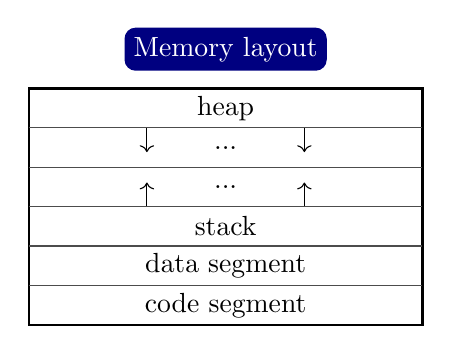
\begin{tikzpicture}
    \memorystack[size x=5cm,word size=1,nb blocks=6,addresses=0]
    \memorypush{code segment}
    \memorypush{data segment}
    \memorypush{stack}
    \memorypush{...}
    \memorypush{...}
    \memorypush{heap}
    \draw[->] (stack3-1.north) ++(-1cm,0) -- +(0,.3cm);
    \draw[->] (stack3-1.north) ++(1cm,0) -- +(0,.3cm);
    \draw[->] (stack6-1.south) ++(-1cm,0) -- +(0,-.3cm);
    \draw[->] (stack6-1.south) ++(1cm,0) -- +(0,-.3cm);
  \end{tikzpicture}
\end{frame}

\begin{frame}[fragile]
  \frametitlecpp[98]{The Stack}
  \begin{block}{Main characteristics}
    \begin{itemize}
    \item allocation on the stack stays valid for the duration of the current scope.
    It is destroyed when it is popped off the stack.
    \item memory allocated on the stack is known at compile time and can thus be accessed through a variable.
    \item the stack is relatively small, it is not a good idea to allocate large arrays, structures or classes
    \item each thread in a process has its own stack
      \begin{itemize}
      \item allocations on the stack are thus ``thread private''
      \item and do not introduce any thread safety issues
      \end{itemize}
    \end{itemize}
  \end{block}
\end{frame}

\begin{frame}[fragile]
  \frametitlecpp[98]{Object allocation on the stack}
  \begin{block}{On the stack}
    \begin{itemize}
    \item objects are created on variable definition (constructor called)
    \item objects are destructed when out of scope (destructor is called)
    \end{itemize}
  \end{block}
  \begin{cppcode}
    int f() {
      MyFirstClass a{3}; // constructor called
      ...
    } // destructor called

    int g() {
      MyFirstClass a; // default constructor called
      ...
    }  // destructor called
  \end{cppcode}
\end{frame}

\begin{frame}[fragile]
  \frametitlecpp[98]{The Heap}
  \begin{block}{Main characteristics}
    \begin{itemize}
    \item Allocated memory stays allocated until it is specifically deallocated
      \begin{itemize}
      \item beware memory leaks
      \end{itemize}
    \item Dynamically allocated memory must be accessed through pointers
    \item large arrays, structures, or classes should be allocated here
    \item there is a single, shared heap per process
      \begin{itemize}
      \item allows to share data between threads
      \item introduces race conditions and thread safety issues!
      \end{itemize}
    \end{itemize}
  \end{block}
\end{frame}

\begin{frame}[fragile]
  \frametitlecpp[98]{Object allocation on the heap}
  \begin{block}{On the heap}
    \begin{itemize}
    \item objects are created by calling \cppinline{new} (constructor is called)
    \item objects are destructed by calling \cppinline{delete} (destructor is called)
    \end{itemize}
  \end{block}
  \begin{cppcode}
    int f() {
      // default constructor called
      MyFirstClass *a = new MyFirstClass;
      delete a; // destructor is called
    }
    int g() {
      // constructor called
      MyFirstClass *a = new MyFirstClass{3};
    } // memory leak !!!
  \end{cppcode}
  \begin{goodpractice}[Prefer smart pointer]{Prefer smart pointers over new/delete}
    Prefer smart pointers to manage objects (discussed later)
  \end{goodpractice}
\end{frame}

\begin{frame}[fragile]
  \frametitlecpp[98]{Array allocation on the heap}
  \begin{block}{Arrays on the heap}
    \begin{itemize}
    \item arrays of objects are created by calling \cppinline{new[]} \\
      default constructor is called for each object of the array
    \item arrays of object are destructed by calling \cppinline{delete[]} \\
      destructor is called for each object of the array
    \end{itemize}
  \end{block}
  \begin{cppcode}
    int f() {
      // default constructor called 10 times
      MyFirstClass *a = new MyFirstClass[10];
      ...
      delete[] a; // destructor called 10 times
    }
  \end{cppcode}
  \begin{goodpractice}[Prefer containers]{Prefer containers over new-ed arrays}
    Prefer containers to manage collections of objects (discussed later)
  \end{goodpractice}
\end{frame}

\subsection[advOO]{Advanced OO}

\begin{frame}[fragile]
  \frametitlecpp[98]{Polymorphism}
  \begin{block}{the concept}
    \begin{itemize}
    \item objects actually have multiple types simultaneously
    \item and can be used as any of them
    \end{itemize}
  \end{block}
  \begin{multicols}{2}
    \begin{cppcode*}{gobble=2}
      Polygon p;

      int f(Drawable & d) {...}
      f(p);  //ok

      try {
        throw p;
      } catch (Shape & e) {
        // will be caught
      }
    \end{cppcode*}
    \columnbreak
    \center
    \begin{overprint}
      \onslide<1>
      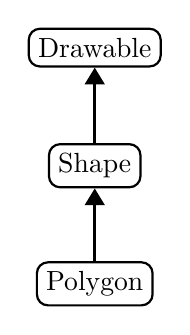
\begin{tikzpicture}[node distance=1.5cm]
        \classbox{Drawable}{}
        \classbox[below of=Drawable]{Shape}{}
        \classbox[below of=Shape]{Polygon}{}
        \draw[very thick,-Triangle] (Polygon) -- (Shape);
        \draw[very thick,-Triangle] (Shape) -- (Drawable);
      \end{tikzpicture}
      \onslide<2->
      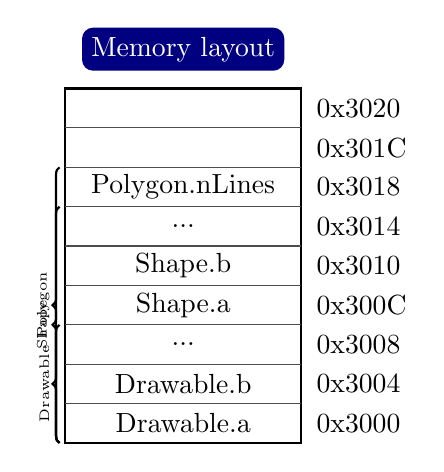
\begin{tikzpicture}
        \memorystack[size x=3cm,word size=1,block size=4,nb blocks=9]
        \memorypush{Drawable.a}
        \memorypush{Drawable.b}
        \memorypush{...}
        \memorypush{Shape.a}
        \memorypush{Shape.b}
        \memorypush{...}
        \memorypush{Polygon.nLines}
        \onslide<2>{\memorystruct{1}{7}{\tiny Polygon}}
        \onslide<3>{\memorystruct{1}{3}{\tiny Drawable}}
        \onslide<4>{\memorystruct{1}{6}{\tiny Shape}}
      \end{tikzpicture}
    \end{overprint}
  \end{multicols}
\end{frame}


\begin{frame}[fragile]
  \frametitlecpp[98]{Inheritance privacy and polymorphism}
  \begin{block}{Only public base classes are visible to outside code}
    \begin{itemize}
    \item private and protected bases are not
    \item this may restrict usage of polymorphism
    \end{itemize}
  \end{block}
  \begin{multicols}{2}
    \begin{cppcode*}{gobble=2}
      Polygon p;

      int f(Drawable & d) {...}
      f(p);  // Not ok anymore

      try {
        throw p;
      } catch (Shape & e) {
        // ok, will be caught
      }
    \end{cppcode*}
    \columnbreak
    \center
    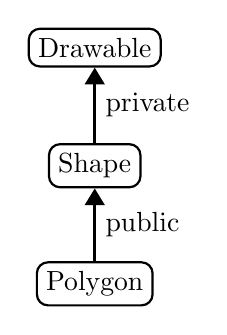
\begin{tikzpicture}[node distance=1.5cm]
      \classbox{Drawable}{}
      \classbox[below of=Drawable]{Shape}{}
      \classbox[below of=Shape]{Polygon}{}
      \draw[very thick,-Triangle] (Polygon) -- (Shape) node[midway,right] {public};
      \draw[very thick,-Triangle] (Shape) -- (Drawable) node[midway,right] {private};
    \end{tikzpicture}
  \end{multicols}
\end{frame}

\begin{frame}[fragile]
  \frametitlecpp[98]{Method overriding}
  \begin{block}{the idea}
    \begin{itemize}
    \item a method of the parent class can be replaced in a derived class
    \item but which one is called?
    \end{itemize}
  \end{block}
  \begin{multicols}{2}
    \begin{cppcode*}{gobble=2}
      Polygon p;
      p.draw(); // ?

      Shape & s = p;
      s.draw(); // ?
    \end{cppcode*}
    \columnbreak
    \center
    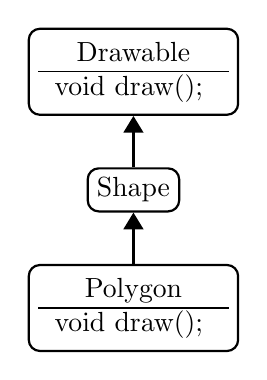
\begin{tikzpicture}[node distance=1.5cm]
      \classbox{Drawable}{
        void draw();
      }
      \classbox[below of=Drawable]{Shape}{}
      \classbox[below of=Shape]{Polygon}{
        void draw();
      }
      \draw[very thick,-Triangle] (Polygon) -- (Shape);
      \draw[very thick,-Triangle] (Shape) -- (Drawable);
    \end{tikzpicture}
  \end{multicols}
\end{frame}

\begin{frame}[fragile]
  \frametitlecpp[98]{Virtual methods}
  \begin{block}{the concept}
    \begin{itemize}
    \item methods can be declared \cppinline{virtual}
    \item for these, the most derived object's implementation is used
          (i.e.\ the dynamic type behind a pointer/reference)
    \item for non-virtual methods, the static type of the variable decides
    \end{itemize}
  \end{block}
  \begin{overprint}
  \onslide<2>
  \begin{multicols}{2}
    \begin{cppcode*}{gobble=2}
      Polygon p;
      p.draw(); // Polygon.draw

      Shape & s = p;
      s.draw(); // Drawable.draw
    \end{cppcode*}
    \columnbreak
    \center
    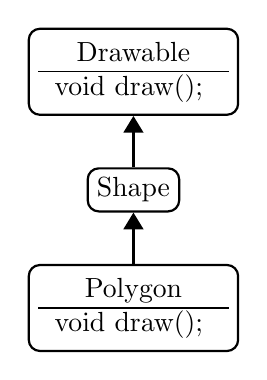
\begin{tikzpicture}[node distance=1.5cm]
      \classbox{Drawable}{
        \cppinline{void draw();}
      }
      \classbox[below of=Drawable]{Shape}{}
      \classbox[below of=Shape]{Polygon}{
        \cppinline{void draw();}
      }
      \draw[very thick,-Triangle] (Polygon) -- (Shape);
      \draw[very thick,-Triangle] (Shape) -- (Drawable);
    \end{tikzpicture}
  \end{multicols}

  \onslide<3>
    \begin{multicols}{2}
    \begin{cppcode*}{gobble=2,highlightlines=5}
      Polygon p;
      p.draw(); // Polygon.draw

      Shape & s = p;
      s.draw(); // Polygon.draw
    \end{cppcode*}
    \columnbreak
    \center
    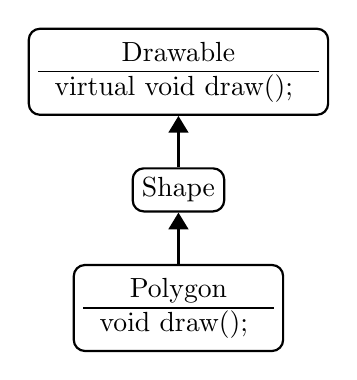
\begin{tikzpicture}[node distance=1.5cm]
      \classbox{Drawable}{
        \cppinline{virtual void draw();}
      }
      \classbox[below of=Drawable]{Shape}{}
      \classbox[below of=Shape]{Polygon}{
        \cppinline{void draw();}
      }
      \draw[very thick,-Triangle] (Polygon) -- (Shape);
      \draw[very thick,-Triangle] (Shape) -- (Drawable);
    \end{tikzpicture}
  \end{multicols}
  \end{overprint}
\end{frame}

\begin{frame}[fragile]
  \frametitlecpp[11]{Virtual methods - implications}
  \begin{block}{Mechanics}
    \begin{itemize}
    \item virtual methods are dispatched at run time
      \begin{itemize}
      \item while non-virtual methods are bound at compile time
      \end{itemize}
    \item they also imply extra storage and an extra indirection
      \begin{itemize}
      \item practically, the object stores a pointer to the correct method
      \item in a so-called ``virtual table'' (``vtable'')
      \end{itemize}
    \end{itemize}
  \end{block}
  \begin{alertblock}{Consequences}
    \begin{itemize}
    \item virtual methods are ``slower'' than standard ones
    \item and they can rarely be inlined
    \item templates are an alternative for performance-critical cases
    \end{itemize}
  \end{alertblock}
\end{frame}

\begin{frame}[fragile]
  \frametitlecpp[11]{{\texttt override} keyword}
  \begin{block}{Principle}
    \begin{itemize}
    \item when overriding a virtual method
    \item the \cppinline|override| keyword should be used
    \item the \cppinline|virtual| keyword is then optional
    \end{itemize}
  \end{block}
  \begin{exampleblock}{Practically}
    \begin{cppcode}
      struct Base {
        virtual void some_func(float);
      };
      struct Derived : Base {
        void some_func(float) override;
      };
    \end{cppcode}
  \end{exampleblock}
\end{frame}

\begin{frame}[fragile]
  \frametitlecpp[11]{Why was {\texttt override} keyword introduced?}
  To detect the mistake in the following code :
  \begin{block}{Without {\texttt override} (\cpp98)}
    \begin{cppcode}
      struct Base {
        virtual void some_func(float);
      };
      struct Derived : Base {
        void some_func(double); // oops !
      };
    \end{cppcode}
  \end{block}
  \begin{itemize}
  \item with \cppinline|override|, you would get a compiler error
  \item if you forget \cppinline|override| when you should have it, you get a compiler warning
  \end{itemize}
\end{frame}

\begin{advanced}
\begin{frame}[fragile]
  \frametitlecpp[11]{{\texttt final} keyword}
  \begin{block}{Idea}
    \begin{itemize}
    \item make sure you cannot further override a given virtual method
    \item by declaring it final
    \end{itemize}
  \end{block}
  \begin{exampleblock}{Practically}
    \begin{cppcode}
      struct Base {
        virtual void some_func(float);
      };
      struct Intermediate : Base {
        void some_func(float) final;
      };
      struct Derived : Intermediate {
        void some_func(float) override; // error
      };
    \end{cppcode}
  \end{exampleblock}
\end{frame}
\end{advanced}

\begin{frame}[fragile]
  \frametitlecpp[11]{Pure Virtual methods}
  \begin{block}{Concept}
    \begin{itemize}
    \item unimplemented methods that must be overridden
    \item marked by \cppinline{= 0} in the declaration
    \item makes their class abstract
    \item only non-abstract classes can be instantiated
    \end{itemize}
  \end{block}
  \pause
  \begin{multicols}{2}
    \begin{cppcode*}{gobble=2}
      // Error : abstract class
      Shape s;

      // ok, draw has been implemented
      Polygon p;

      // Shape type still usable
      Shape & s = p;
      s.draw();
    \end{cppcode*}
    \columnbreak
    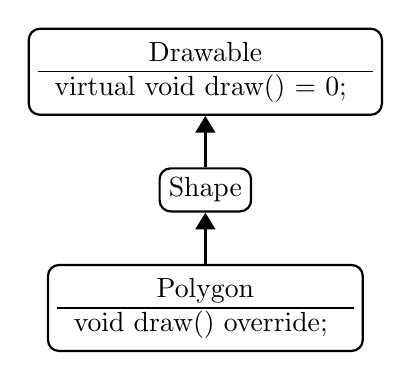
\begin{tikzpicture}[node distance=1.5cm]
      \classbox{Drawable}{
        \cppinline{virtual void draw() = 0;}
      }
      \classbox[below of=Drawable]{Shape}{}
      \classbox[below of=Shape]{Polygon}{
        \cppinline{void draw() override;}
      }
      \draw[very thick,-Triangle] (Polygon) -- (Shape);
      \draw[very thick,-Triangle] (Shape) -- (Drawable);
    \end{tikzpicture}
  \end{multicols}
\end{frame}

\begin{frame}[fragile]
  \frametitlecpp[98]{Polymorphism and destruction}
  \begin{block}{Owning base pointers}
    We sometimes need to maintain owning pointers to base classes:
  \end{block}
  \begin{overprint}
    \onslide<1>
  \begin{cppcode}
    struct Drawable {
       virtual void draw() = 0;
    };
    Drawable* getImpl();

    Drawable* p = getImpl();
    p->draw();
    delete p;
  \end{cppcode}
    \onslide<2>
  \begin{cppcode}
    struct Drawable {
       virtual void draw() = 0;
    };
    std::unique_ptr<Drawable> getImpl(); // better API

    auto p = getImpl();
    p->draw();
  \end{cppcode}
  \end{overprint}
  \begin{block}{}
    \begin{itemize}
      \item What happens when \cppinline{p} is deleted?
      \item What if a class deriving from \cppinline{Drawable} has a destructor?
    \end{itemize}
  \end{block}
\end{frame}

\begin{frame}[fragile]
  \frametitlecpp[11]{Polymorphism and destruction}
  \begin{block}{Virtual destructors}
    \begin{itemize}
    \item We can mark a destructor as \cppinline{virtual}
    \item This selects the right destructor based on the runtime type
    \end{itemize}
  \end{block}
  \begin{cppcode}
    struct Drawable {
       virtual ~Drawable() = default;
       virtual void draw() = 0;
    };
    Drawable* p = getImpl(); // returns derived obj.
    p->draw();
    delete p; // dynamic dispatch to right destructor
  \end{cppcode}
  \begin{goodpractice}{Virtual destructors}
    If you expect users to inherit from your class and override methods (i.e.\ use your class polymorphically), declare its destructor \cppinline{virtual}
  \end{goodpractice}
\end{frame}

\begin{frame}[fragile]
  \frametitlecpp[11]{Pure Abstract Class aka Interface}
  \begin{block}{Definition of pure abstract class}
    \begin{itemize}
    \item a class that has
      \begin{itemize}
        \item no data members
        \item all its methods pure virtual
        \item a \cppinline{virtual} destructor
      \end{itemize}
    \item the equivalent of an Interface in Java
    \end{itemize}
  \end{block}
  \begin{multicols}{2}
    \begin{cppcode*}{gobble=2}
      struct Drawable {
        virtual ~Drawable()
                      = default;
        virtual void draw() = 0;
      }
    \end{cppcode*}
    \columnbreak
    \center
    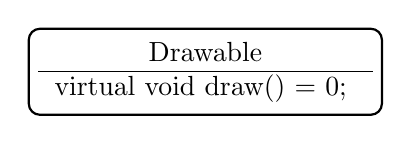
\begin{tikzpicture}[node distance=1.5cm]
      \classbox{Drawable}{
        virtual void draw() = 0;
      }
    \end{tikzpicture}
  \end{multicols}
\end{frame}

\begin{frame}[fragile]
  \frametitlecpp[98]{Overriding overloaded methods}
  \begin{block}{Concept}
    \begin{itemize}
    \item overriding an overloaded method will hide the others
    \item unless you inherit them using \cppinline{using}
    \end{itemize}
  \end{block}
  \begin{cppcode*}{gobble=0}
    struct BaseClass {
      virtual int foo(std::string);
      virtual int foo(int);
    };
    struct DerivedClass : BaseClass {
      using BaseClass::foo;
      int foo(std::string) override;
    };
    DerivedClass dc;
    dc.foo(4);      // error if no using
    \end{cppcode*}
\end{frame}

\begin{frame}[fragile]
  \frametitlecpp[98]{Polymorphism}
  \begin{exercise}{Polymorphism}
    \begin{itemize}
    \item go to \texttt{exercises/polymorphism}
    \item look at the code
    \item open trypoly.cpp
    \item create a Pentagon, call its perimeter method
    \item create a Hexagon, call its perimeter method
    \item create a Hexagon, call its parent's perimeter method
    \item retry with virtual methods
    \end{itemize}
  \end{exercise}
\end{frame}

\begin{frame}[fragile]
  \frametitlecpp[98]{Multiple Inheritance}
  \begin{block}{Concept}
    \begin{itemize}
    \item one class can inherit from multiple parents
    \end{itemize}
  \end{block}
  \begin{multicols}{2}
    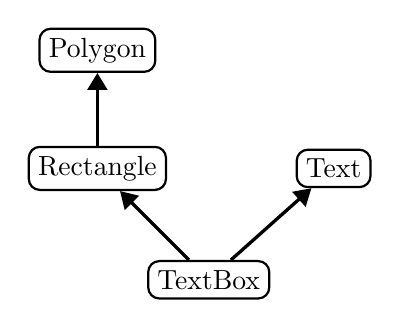
\begin{tikzpicture}[]
      \classbox[]{Polygon}{}
      \classbox[below of=Polygon,node distance=1.5cm]{Rectangle}{}
      \classbox[right of=Rectangle,node distance=3cm]{Text}{}
      \classbox[below right of=Rectangle,node distance=2cm]{TextBox}{}
      \draw[very thick,Triangle-] (Polygon) -- (Rectangle);
      \draw[very thick,Triangle-] (Rectangle) -- (TextBox);
      \draw[very thick,Triangle-] (Text) -- (TextBox);
    \end{tikzpicture}
    \columnbreak
    \vspace{2cm}
    \begin{cppcode*}{gobble=2}
      class TextBox :
        public Rectangle, Text {
        // inherits from both
        // publicly from Rectangle
        // privately from Text
      }
    \end{cppcode*}
  \end{multicols}
\end{frame}

\begin{frame}[fragile]
  \frametitlecpp[98]{The diamond shape}
  \begin{block}{Definition}
    \begin{itemize}
    \item situation when one class inherits several times from a given grand parent
    \end{itemize}
  \end{block}
  \begin{alertblock}{Problem}
    \begin{itemize}
    \item are the members of the grand parent replicated?
    \end{itemize}
  \end{alertblock}
  \vfill
  \hspace{2.5cm}
  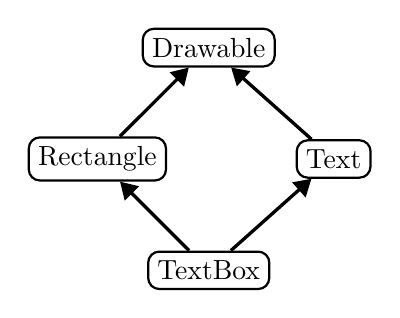
\begin{tikzpicture}[]
    \classbox[]{Drawable}{}
    \classbox[below left of=Drawable,node distance=2cm]{Rectangle}{}
    \classbox[right of=Rectangle,node distance=3cm]{Text}{}
    \classbox[below right of=Rectangle,node distance=2cm]{TextBox}{}
    \draw[very thick,Triangle-] (Drawable) -- (Rectangle);
    \draw[very thick,Triangle-] (Drawable) -- (Text);
    \draw[very thick,Triangle-] (Rectangle) -- (TextBox);
    \draw[very thick,Triangle-] (Text) -- (TextBox);
  \end{tikzpicture}
\end{frame}

\begin{frame}[fragile]
  \frametitlecpp[98]{Virtual inheritance}
  \begin{block}{Solution}
    \begin{itemize}
    \item inheritance can be \cppinline{virtual} or not
    \begin{itemize}
      \item \cppinline{virtual} inheritance will ``share'' parents
      \item standard inheritance will replicate them
    \end{itemize}
    \item most derived class will call the virtual base class's constructor
    \end{itemize}
    \begin{cppcode}
      class Text : public virtual Drawable {...};
      class Rectangle : public virtual Drawable {...};
    \end{cppcode}
  \end{block}
  \begin{multicols}{2}
    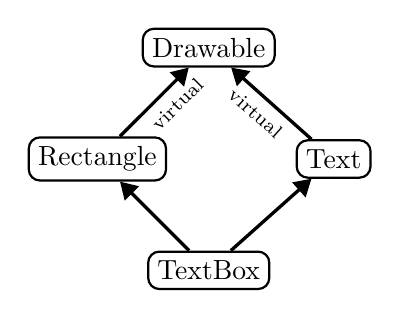
\begin{tikzpicture}[]
      \classbox{Drawable}{}
      \classbox[below left of=Drawable,node distance=2cm]{Rectangle}{}
      \classbox[right of=Rectangle,node distance=3cm]{Text}{}
      \classbox[below right of=Rectangle,node distance=2cm]{TextBox}{}
      \draw[very thick,Triangle-] (Drawable) -- node[below,pos=0.35,sloped] {\scriptsize virtual} (Rectangle);
      \draw[very thick,Triangle-] (Drawable) -- node[below,pos=0.45,sloped] {\scriptsize virtual} (Text);
      \draw[very thick,Triangle-] (Rectangle) -- (TextBox);
      \draw[very thick,Triangle-] (Text) -- (TextBox);
    \end{tikzpicture}
    \columnbreak
    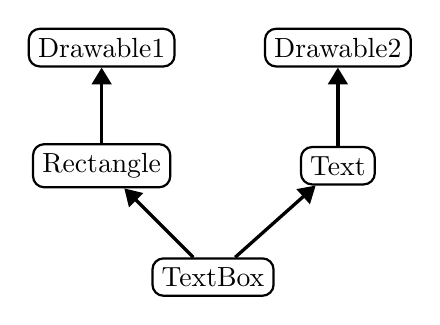
\begin{tikzpicture}[]
      \classbox[]{Drawable1}{}
      \classbox[below of=Drawable1,node distance=1.5cm]{Rectangle}{}
      \draw[very thick,Triangle-] (Drawable1) -- (Rectangle);
      \classbox[right of=Drawable1,node distance=3cm]{Drawable2}{}
      \classbox[below of=Drawable2,node distance=1.5cm]{Text}{}
      \draw[very thick,Triangle-] (Drawable2) -- (Text);
      \classbox[below right of=Rectangle,node distance=2cm]{TextBox}{}
      \draw[very thick,Triangle-] (Rectangle) -- (TextBox);
      \draw[very thick,Triangle-] (Text) -- (TextBox);
    \end{tikzpicture}
  \end{multicols}
\end{frame}

\begin{frame}[fragile]
  \frametitlecpp[98]{Multiple inheritance advice}
  \begin{goodpractice}{Avoid multiple inheritance}
    \begin{itemize}
    \item Except for inheriting from interfaces
    \item And for rare special cases
    \end{itemize}
  \end{goodpractice}
  \begin{goodpractice}[NO diamond inheritance]{Absolutely avoid diamond-shaped inheritance}
    \begin{itemize}
    \item This is a sign that your architecture is not correct
    \item In case you are tempted, think twice and change your mind
    \end{itemize}
  \end{goodpractice}
\end{frame}

\begin{frame}[fragile]
  \frametitlecpp[98]{Virtual inheritance}
  \begin{exerciseWithShortcut}{Virtual inheritance}{Virtual OO}
    \begin{itemize}
    \item go to \texttt{exercisescode/virtual\_inheritance}
    \item look at the code
    \item open trymultiherit.cpp
    \item create a TextBox and call draw
    \item Fix the code to call both draws by using types
    \item retry with virtual inheritance
    \end{itemize}
  \end{exerciseWithShortcut}
\end{frame}

\begin{advanced}
  \input{objectorientation/typecasting}
\end{advanced}
\input{objectorientation/operators}
\input{objectorientation/functors}
\begin{advanced}
  \input{objectorientation/adl}
\end{advanced}

\section[More]{Core modern \cpp}
\input{morelanguage/constness}
\begin{advanced}
  \input{morelanguage/constexpr}
\end{advanced}
\input{morelanguage/exceptions}
\begin{advanced}
  \input{morelanguage/move}
  \input{morelanguage/copyelision}
\end{advanced}
\input{morelanguage/templates}
\input{morelanguage/lambda}
\subsection[STL]{The STL}

\begin{frame}[fragile]
  \frametitlecpp[98]{The Standard Template Library}
  \begin{block}{What it is}
    \begin{itemize}
    \item A library of standard templates
    \item Has almost everything you need
      \begin{itemize}
      \item strings, containers, iterators
      \item algorithms, functions, sorters
      \item functors, allocators
      \item ...
      \end{itemize}
    \item Portable
    \item Reusable
    \item Efficient
    \end{itemize}
  \end{block}
  \pause
  \begin{exampleblock}{Use it}
    and adapt it to your needs, thanks to templates
  \end{exampleblock}
\end{frame}

\begin{frame}[fragile]
  \frametitlecpp[14]{STL in practice}
  \begin{exampleblockGB}{STL example}{https://godbolt.org/z/n8ahEr5f6}{STL}
    \begin{cppcode*}{gobble=2}
      #include <vector>
      #include <algorithm>
      #include <functional>     // `import std;` in C++23
      #include <iterator>
      #include <iostream>

      std::vector<int> in{5, 3, 4};    // initializer list
      std::vector<int> out(3);  // constructor taking size
      std::transform(in.begin(), in.end(),  // input range
                     out.begin(),          // start result
                     std::negate{});       // function obj
      std::copy(out.begin(), out.end(),    // -5 -3 -4
        std::ostream_iterator<int>{std::cout, " "});
    \end{cppcode*}
  \end{exampleblockGB}
\end{frame}

\begin{frame}[fragile]
  \frametitlecpp[98]{STL's concepts}
  \begin{block}{containers}
    \small
    \begin{itemize}
    \setlength\itemsep{0em}
    \setlength{\parskip}{0pt}
    \setlength{\parsep}{0pt}
    \item data structures for managing a range of elements, irrespective of:
      \begin{itemize}
      \setlength\itemsep{0em}
      \setlength{\parskip}{0pt}
      \setlength{\parsep}{0pt}
      \item the data itself (templated)
      \item the memory allocation of the structure (templated)
      \item the algorithms that may use the structure (iterators)
      \end{itemize}
    \end{itemize}
  \end{block}
  \begin{exampleblock}{Examples ($\rightarrow$ \href{https://en.cppreference.com/w/cpp/string/basic_string}{\color{blue!50!white}{string}} and \href{https://en.cppreference.com/w/cpp/container}{\color{blue!50!white}{container library}} on cppreference)}
    \small
    \begin{itemize}
      \setlength\itemsep{0em}
      \item string, string\_view (\cpp17)
      \item list, forward\_list (\cpp11), vector, deque, array (\cpp11)
      \item {[}multi]map, [multi]set (\cpp23: flat\_[multi]map, flat\_[multi]set)
      \item unordered\_[multi]map (\cpp11), unordered\_[multi]set (\cpp11)
      \item stack, queue, priority\_queue
      \item span (\cpp20)
      \item non-containers: bitset, pair, tuple (\cpp11), optional (\cpp17), variant (\cpp17), any (\cpp17), expected (\cpp23)
    \end{itemize}
  \end{exampleblock}
\end{frame}

\begin{frame}[fragile]
  \frametitlecpp[11]{Containers: std::vector}
  \begin{cppcode*}{}
    #include <vector>
    std::vector<T> v{5, 3, 4}; // 3 Ts, 5, 3, 4
    std::vector<T> v(100);     // 100 default constr. Ts
    std::vector<T> v(100, 42); // 100 Ts with value 42
    std::vector<T> v2 = v;            // copy
    std::vector<T> v2 = std::move(v); // move, v is empty

    std::size_t s = v.size();
    bool empty = v.empty();

    v[2] = 17;         // write element 2
    T& t = v[1000];    // access element 1000, bug!
    T& t = v.at(1000); // throws std::out_of_range
    T& f = v.front();  // access first element
    v.back() = 0;      // write to last element
    T* p = v.data();   // pointer to underlying storage
  \end{cppcode*}
\end{frame}

\begin{frame}[fragile]
  \frametitlecpp[11]{Containers: std::vector}
  \begin{cppcode*}{}
    std::vector<T> v = ...;
    auto b = v.begin(); // iterator to first element
    auto e = v.end();   // iterator to one past last element
    // all following operations, except reserve, invalidate
    // all iterators (b and e) and references to elements

    v.resize(100); // size changes, grows: new T{}s appended
                   //           shrinks: Ts at end destroyed
    v.reserve(1000); // size remains, memory increased
    for (T i = 0; i < 900; i++)
      v.push_back(i); // add to the end
    v.insert(v.begin()+3, T{}); // insert after 3rd position

    v.pop_back();         // removes last element
    v.erase(v.end() - 3); // removes 3rd-last element
    v.clear();            // removes all elements
  \end{cppcode*}
\end{frame}

\begin{frame}[fragile]
    \frametitlecpp[11]{Containers: \texttt{std::unordered\_map}}
    \begin{block}{}
        Conceptually a container of \cppinline{std::pair<Key const, Value>}
    \end{block}
    \begin{cppcode*}{gobble=4}
        #include <unordered_map>
        std::unordered_map<std::string, int> m;
        m["hello"] = 1;  // inserts new key, def. constr. value
        m["hello"] = 2;  // finds existing key
        auto [it, isNewKey] = m.insert({"hello", 0}); // no effect
        int val = m["world"];    // inserts new key (val == 0)
        int val = m.at("monde"); // throws std::out_of_range

        if (auto it = m.find("hello"); it != m.end()) // C++17
            m.erase(it);      // remove by iterator (fast)
        if (m.contains("hello")) // C++20
            m.erase("hello"); // remove by key, 2. lookup, bad
        for (auto const& [k, v] : m) // iterate k/v pairs (C++17)
            std::cout << k << ": " << v << '\n';
    \end{cppcode*}
\end{frame}

\begin{frame}[fragile]
    \frametitlecpp[11]{\texttt{std::hash}}
    \begin{block}{}
        \begin{itemize}
            \item The standard utility to create hash codes
            \item Used by \cppinline{std::unordered_map} and others
            \item Can be customized for your types via template specialization
        \end{itemize}
    \end{block}
    \begin{cppcode*}{gobble=4}
        #include <functional>
        std::hash<std::string> h;
        std::cout << h("hello"); // 2762169579135187400
        std::cout << h("world"); // 8751027807033337960

        class MyClass { int a, b; ... };
        template<> struct std::hash<MyClass> {
          std::size_t operator()(MyClass const& c) {
            std::hash<int> h;
            return h(c.a) ^ h(c.b); // xor to combine hashes
          }
        };
    \end{cppcode*}
\end{frame}

\begin{frame}[fragile]
  \frametitlecpp[11]{STL's concepts}
  \begin{block}{iterators}
    \begin{itemize}
    \item generalization of pointers
    \item allow iteration over some data, irrespective of:
      \begin{itemize}
      \item the container used (templated)
      \item the data itself (container is templated)
      \item the consumer of the data (templated algorithm)
      \end{itemize}
    \item examples
      \begin{itemize}
        \item \cppinline{std::reverse_iterator}, \cppinline{std::back_insert_iterator}, ...
      \end{itemize}
    \end{itemize}
  \end{block}
  \begin{exampleblockGB}{Iterator example}{https://godbolt.org/z/jv1qTo5xz}{Iterator example}
    \begin{cppcode*}{}
      std::vector<int> const v = {1,2,3,4,5,6,7,8,9};
      auto const end = v.rend() - 3; // arithmetic
      for (auto it = v.rbegin();
           it != end;     // compare positions
           it += 2)       // jump 2 positions
        std::cout << *it; // dereference, prints: 975
    \end{cppcode*}
  \end{exampleblockGB}
\end{frame}

\begin{frame}[fragile]
  \frametitlecpp[98]{STL's concepts}
  \begin{block}{algorithms}
    \begin{itemize}
    \item implementation of an algorithm working on data
    \item with a well defined behavior (defined complexity)
    \item irrespective of
      \begin{itemize}
      \item the data handled
      \item the container where the data live
      \item the iterator used to go through data (almost)
      \end{itemize}
    \item examples
      \begin{itemize}
      \item for\_each, find, find\_if, count, count\_if, search
      \item copy, swap, transform, replace, fill, generate
      \item remove, remove\_if
      \item unique, reverse, rotate, shuffle, partition
      \item sort, partial\_sort, merge, make\_heap, min, max
      \item lexicographical\_compare, iota, reduce, partial\_sum
      \end{itemize}
    \item see also \href{https://www.youtube.com/watch?v=2olsGf6JIkU}{105 STL Algorithms in Less Than an Hour} and the \href{https://en.cppreference.com/w/cpp/algorithm}{algorithms library} on cppreference
    \end{itemize}
  \end{block}
\end{frame}

\begin{frame}[fragile]
  \frametitlecpp[98]{STL's concepts}
  \begin{block}{functors / function objects}
    \begin{itemize}
      \item generic utility functions
      \item as structs with \cppinline{operator()}
      \item mostly useful to be passed to STL algorithms
    \item implemented independently of
      \begin{itemize}
      \item the data handled (templated)
      \item the context (algorithm) calling it
      \end{itemize}
    \item examples
      \begin{itemize}
      \item plus, minus, multiplies, divides, modulus, negate
      \item equal\_to, less, greater, less\_equal, ...
      \item logical\_and, logical\_or, logical\_not
      \item bit\_and, bit\_or, bit\_xor, bit\_not
      \item identity, not\_fn
      \item bind, bind\_front
      \end{itemize}
    \item see also documentation on \href{https://en.cppreference.com/w/cpp/utility/functional}{cppreference}
    \end{itemize}
  \end{block}
\end{frame}

\begin{frame}[fragile]
  \frametitlecpp[11]{Functors / function objects}
  \begin{block}{Example}
    \begin{cppcode*}{}
      struct Incrementer {
        int m_inc;
        Incrementer(int inc) : m_inc(inc) {}

        int operator()(int value) const {
          return value + m_inc;
        }
      };
      std::vector<int> v{1, 2, 3};
      const auto inc = 42;
      std::transform(v.begin(), v.end(), v.begin(),
                     Incrementer{inc});
      \end{cppcode*}
    \end{block}
\end{frame}

\begin{frame}[fragile]
  \frametitlecpp[11]{Prefer lambdas over functors}
  \begin{exampleblock}{With lambdas}
    \begin{cppcode*}{}
      std::vector<int> v{1, 2, 3};
      const auto inc = 42;
      std::transform(begin(v), end(v), begin(v),
                     [inc](int value) {
                       return value + inc;
                     });
    \end{cppcode*}
  \end{exampleblock}
  \pause
  \begin{goodpractice}[STL and lambdas]{Use STL algorithms with lambdas}
    \begin{itemize}
      \item Prefer lambdas over functors when using the STL
      \item Avoid binders like \cppinline{std::bind2nd}, \cppinline{std::ptr_fun}, etc.
    \end{itemize}
  \end{goodpractice}
\end{frame}

\begin{frame}[fragile]
  \frametitlecpp[11]{Range-based for loops with STL containers}
  \begin{block}{Iterator-based loop (since \cpp98)}
    \begin{cppcode*}{}
      std::vector<int> v = ...;
      int sum = 0;
      for (std::vector<int>::iterator it = v.begin();
           it != v.end(); it++)
        sum += *it;
    \end{cppcode*}
  \end{block}
  \pause
  \begin{block}{Range-based for loop (since \cpp11)}
    \begin{cppcode*}{firstnumber=6}
      std::vector<int> v = ...;
      int sum = 0;
      for (auto a : v) { sum += a; }
    \end{cppcode*}
  \end{block}
  \pause
  \begin{exampleblock}{STL way (since \cpp98)}
    \begin{cppcode*}{firstnumber=9}
      std::vector<int> v = ...;
      int sum = std::accumulate(v.begin(), v.end(), 0);
      // std::reduce(v.begin(), v.end()); // C++17
    \end{cppcode*}
  \end{exampleblock}
\end{frame}

\begin{frame}[fragile]
  \frametitlecpp[17]{More examples}
  \begin{cppcode}
    std::list<int> l = ...;

    // Finds the first element in a list between 1 and 10.
    const auto it = std::find_if(l.begin(), l.end(),
        [](int i) { return i >= 1 && i <= 10; });
    if (it != l.end()) {
      int element = *it; ...
    }

    // Computes sin(x)/(x + DBL_MIN) for elements of a range.
    std::vector<double> r(l.size());
    std::transform(l.begin(), l.end(), r.begin(),
      [](auto x) { return std::sin(x)/(x + DBL_MIN); });

    // reduce/fold (using addition)
    const auto sum = std::reduce(v.begin(), v.end());
  \end{cppcode}
\end{frame}

\begin{frame}[fragile]
  \frametitlecpp[11]{More examples}
  \begin{cppcode}
    std::vector<int> v = ...;

    // remove duplicates
    std::sort(v.begin(), v.end());
    auto newEndIt = std::unique(v.begin(), v.end());
    v.erase(newEndIt, v.end());

    // remove by predicate
    auto p = [](int i) { return i > 42; };
    auto newEndIt = std::remove_if(v.begin(), v.end(), p);
    v.erase(newEndIt, v.end());

    // remove by predicate (C++20)
    std::erase_if(v, p);
  \end{cppcode}
\end{frame}

\begin{frame}[fragile]
  \frametitlecpp[98]{Welcome to lego programming!}
  \begin{block}{}
    \pgfdeclareimage[height=0.5cm]{AtlasLego}{morelanguage/AtlasLego.jpg}
    \includegraphics[width=\linewidth]{morelanguage/AtlasLego}
  \end{block}
\end{frame}

\begin{frame}[fragile]
  \frametitlecpp[98]{Using the STL}
  \begin{exercise}{STL}
    \begin{itemize}
    \item go to \texttt{exercises/stl}
    \item look at the non STL code in randomize.nostl.cpp
      \begin{itemize}
        \item it creates a vector of ints at regular intervals
        \item it randomizes them
        \item it computes differences between consecutive ints
        \item and the mean and variance of it
      \end{itemize}
    \item open randomize.cpp and complete the ``translation'' to STL
    \item see how easy it is to reuse the code with complex numbers
    \end{itemize}
  \end{exercise}
\end{frame}

\begin{frame}[fragile]
  \frametitlecpp[98]{Using the STL}
  \begin{exampleblock}{Be brave and persistent!}
    \begin{itemize}
    \item you may find the STL quite difficult to use
    \item template syntax is really tough
    \item it is hard to get right, compilers spit out long error novels
    \begin{itemize}
      \item but, compilers are getting better with error messages
    \end{itemize}
    \item \cpp20 will help with concepts and ranges
    \item the STL is extremely powerful and flexible
    \item it will be worth your time!
    \end{itemize}
  \end{exampleblock}
\end{frame}

\begin{advanced}
  \input{morelanguage/morestl}
  %\subsection[rnd]{Random}

\begin{frame}[fragile]
  \frametitlecpp[11]{Pseudo-random number generators (PRNG)}
  \begin{block}{Concept}
    \begin{itemize}
      \item For generating pseudo-random numbers the STL offers:
      \begin{itemize}
        \item engines and engine adaptors to generate pseudo random bits
        \item distributions to shape these into numbers
        \item access to (potential) hardware entropy
      \end{itemize}
      \item All found in header \cppinline{<random>}
    \end{itemize}
  \end{block}
  \begin{exampleblock}{Example}
    \begin{cppcode}
      #include <random>
      std::random_device rd;
      std::default_random_engine engine{rd()};
      std::normal_distribution dist(5.0, 1.5); // µ, σ
      double r = dist(engine);
    \end{cppcode}
  \end{exampleblock}
\end{frame}

\begin{frame}[fragile]
  \frametitlecpp[11]{Engines}
  \begin{block}{Engines}
    \begin{itemize}
      \item Generate random bits (as integers), depending on algorithm
      \item Can be seeded via constructor or \cppinline{seed()}
      \item Algorithms:
        {\footnotesize \cppinline{linear_congruential_engine}, \cppinline{mersenne_twister_engine}, \cppinline{subtract_with_carry_engine}}
      \item Adaptors:
        {\footnotesize \cppinline{discard_block_engine}, \cppinline{independent_bits_engine}, \cppinline{shuffle_order_engine}}
      \item Aliases:
        {\footnotesize \cppinline{minstd_rand0}, \cppinline{minstd_rand}, \cppinline{mt19937}, \cppinline{mt19937_64}, \cppinline{ranlux24}, \cppinline{ranlux48}, \cppinline{knuth_b}} (use these)
      \item \cppinline{std::default_random_engine} aliases one of the above
    \end{itemize}
  \end{block}
  \begin{exampleblock}{Engine creation with seed}
    \begin{cppcode}
      std::default_random_engine engine{42}; // or empty
      auto i = engine(); // operator(): random integer
    \end{cppcode}
  \end{exampleblock}
\end{frame}

\begin{frame}[fragile]
  \frametitlecpp[11]{Determinism and random device}
  \begin{block}{Engines / PRNGs}
    \begin{itemize}
      \item Are \emph{deterministic}
      \item Will produce the same number sequence for the same seed
      \item May be useful for reproducibility
    \end{itemize}
  \end{block}
  \begin{block}{\texttt{std::random\_device}}
    \begin{itemize}
      \item Provides \emph{non-deterministic} random numbers
      \item Uses hardware provided entropy, if available
      \item May become slow when called too often,\\e.g.\ when hardware entropy pool is exhausted
      \item Use only to seed engine, if \emph{non-deterministic} numbers needed
    \end{itemize}
  \end{block}
  \begin{exampleblock}{Non-deterministic engine seeding}
    \begin{cppcode}
      std::random_device rd;
      std::default_random_engine engine{rd()};
    \end{cppcode}
  \end{exampleblock}
\end{frame}

\begin{frame}[fragile]
  \frametitlecpp[11]{Distributions}
  \begin{block}{Distributions}
    \begin{itemize}
      \item Take random bits from engines and shape them into numbers
      \item Standard library provides a lot of them
      \begin{itemize}
        \item Uniform, bernoulli, poisson, normal and sampling distributions
        \item See \href{https://en.cppreference.com/w/cpp/numeric/random}{cppreference} for the full list
      \end{itemize}
    \end{itemize}
  \end{block}
  \begin{exampleblock}{Distributions sharing a non-deterministic engine}
    \begin{cppcode*}{gobble=2}
      std::random_device rd;
      std::default_random_engine engine{rd()};
      std::uniform_int_distribution<int> dist(2,7);//min,max
      const int size = dist(engine); // gen. random number
      std::vector<int> v(size);
      std::normal_distribution<double> norm(5.0, 1.5); //µ,σ
      std::generate(begin(v), end(v),
                    [&]{ return norm(engine); });
    \end{cppcode*}
  \end{exampleblock}
\end{frame}

\begin{frame}[fragile]
  \frametitlecpp[98]{C random library}
  \begin{block}{C random library}
    \begin{itemize}
      \item The C library (\cppinline{<cstdlib>}) offers a primitive PRNG:
      \item \cppinline{rand()} returns random int between 0 and \cppinline{RAND_MAX} (incl.)
      \item \cppinline{srand(seed)} sets the global seed
    \end{itemize}
  \end{block}
  \begin{alertblock}{Disadvantages}
    \begin{itemize}
      \item Seeding is not thread-safe; \cppinline{rand()} may be.
      \item Returned numbers have small, implementation-defined range
      \item No guarantee on quality
      \item Mapping a random number to a custom range is hard
      \item E.g.: \cppinline{rand() % 10} yields biased numbers and is wrong!
    \end{itemize}
  \end{alertblock}
  \begin{goodpractice}[C random library]{Strongly avoid the C random library}
    Use the \cpp11 facilities from the \cppinline{<random>} header
  \end{goodpractice}
\end{frame}

  \input{morelanguage/ranges}
\end{advanced}
\subsection[RAII]{RAII and smart pointers}

\begin{frame}[fragile]
  \frametitlecpp[98]{Pointers: why are they error prone?}
  \begin{exampleblock}{They need initialization
      \hfill \onslide<2->{\textcolor{orange}{\bf Seg Fault}}}
    \begin{cppcode*}{xleftmargin=20pt}
      char *s;
      try {
        foo(); // may throw
        s = new char[100];
        read_line(s);
      } catch (...) { ... }
      process_line(s);
    \end{cppcode*}
  \end{exampleblock}
  \pause
  \pause
  \vspace{-2cm}
  \begin{exampleblock}{They need to be released
      \hfill \onslide<4->{\textcolor{orange}{\bf Memory leak}}}
    \begin{cppcode*}{xleftmargin=20pt}
      char *s = new char[100];
      read_line(s);
      if (s[0] == '#') return;
      process_line(s);
      delete[] s;
    \end{cppcode*}
  \end{exampleblock}
  \pause
  \pause
  \vspace{-2cm}
  \begin{exampleblock}{They need clear ownership
      \hfill \onslide<6->{\textcolor{orange}{\bf Who should release ?}}}
    \begin{cppcode*}{xleftmargin=20pt}
      char *s = new char[100];
      read_line(s);
      vec.push_back(s);
      set.add(s);
      std::thread t1{func1, vec};
      std::thread t2{func2, set};
    \end{cppcode*}
  \end{exampleblock}
\end{frame}

\begin{frame}[fragile]
  \frametitlecpp[11]{This problem exists for any resource}
  \begin{exampleblock}{For example with a file}
    \begin{cppcode*}{}
      std::FILE *handle = std::fopen(path, "w+");
      if (nullptr == handle) { throw ... }
      std::vector v(100, 42);
      write(handle, v);
      if (std::fputs("end", handle) == EOF) {
        return;
      }
      std::fclose(handle);
    \end{cppcode*}
  \end{exampleblock}
  \begin{block}{}
    Which problems do you spot in the above snippet?
  \end{block}
\end{frame}

\begin{frame}
  \frametitlecpp[98]{Resource Acquisition Is Initialization (RAII)}
  \begin{block}{Practically}
    Use variable construction/destruction and scope semantics:
    \begin{itemize}
    \item wrap the resource inside a class
    \item acquire resource in constructor
    \item release resource in destructor
    \item create an instance on the stack
    \begin{itemize}
      \item automatically destructed when leaving the scope
      \item including in case of exception
    \end{itemize}
    \item use move semantics to pass the resource around
    \end{itemize}
  \end{block}
\end{frame}

\begin{frame}[fragile]
  \frametitlecpp[98]{RAII in practice}
  \begin{exampleblock}{An RAII File class}
    \small
    \begin{cppcode*}{gobble=2}
      class File {
      public:
        // constructor: acquire resource
        File(const char* filename)
          : m_handle(std::fopen(filename, "w+")) {
          // abort constructor on error
          if (m_handle == nullptr) { throw ... }
        }
        // destructor: release resource
        ~File() { std::fclose(m_handle); }
        void write (const char* str) {
          ...
        }
      private:
        std::FILE* m_handle; // wrapped resource
      };
    \end{cppcode*}
  \end{exampleblock}
\end{frame}

\begin{frame}[fragile]
  \frametitlecpp[98]{RAII usage}
  \begin{exampleblock}{Usage of File class}
    \begin{cppcode*}{}
      void log_function() {
        // file opening, aka resource acquisition
        File logfile("logfile.txt");

        // file usage
        logfile.write("hello logfile!"); // may throw

        // file is automatically closed by the call to
        // its destructor, even in case of exception!
      }
    \end{cppcode*}
  \end{exampleblock}
  \begin{goodpractice}[Use \texttt{std::fstream}]{Use \texttt{std::fstream} for file handling}
     The standard library provides \cppinline{std::fstream} to handle files, use it!
  \end{goodpractice}
\end{frame}

\begin{frame}[fragile]
  \frametitlecpp[11]{\texttt{std::unique\_ptr}}
  \begin{block}{A RAII pointer}
    \begin{itemize}
    \item wraps and behaves like a regular pointer
    \item get underlying pointer using \cppinline{get()}
    \item when destroyed, deletes the object pointed to
    \item has move-only semantic
      \begin{itemize}
      \item the pointer has unique ownership
      \item copying will result in a compile error
      \end{itemize}
    \end{itemize}
  \end{block}
  \pause
  \begin{exampleblock}{}
    \begin{cppcode*}{}
      #include <memory>
      void f(std::unique_ptr<Foo> ptr) {
        ptr->bar();
      } // deallocation when f exits

      std::unique_ptr<Foo> p{ new Foo{} }; // allocation
      f(std::move(p)); // transfer ownership
      assert(p.get() == nullptr);
    \end{cppcode*}
  \end{exampleblock}
\end{frame}

\begin{frame}[fragile]
  \frametitlecpp[11]{Quiz}
  \begin{exampleblock}{What do you expect?}
    \begin{cppcode*}{}
      void f(std::unique_ptr<Foo> ptr);
      std::unique_ptr<Foo> uptr(new Foo{});
      f(uptr); // transfer of ownership
    \end{cppcode*}
  \end{exampleblock}
  \pause
  \begin{alertblock}{Compilation Error - \godboltLink{https://godbolt.org/z/jfqKjocnh}{\texttt{unique\_ptr} copy}}
    \begin{minted}{text}
test.cpp:15:5: error: call to deleted constructor
of 'std::unique_ptr<Foo>'
  f(uptr);
    ^~~~
/usr/include/c++/4.9/bits/unique_ptr.h:356:7: note:
 'unique_ptr' has been explicitly marked deleted here
 unique_ptr(const unique_ptr&) = delete;
 ^
    \end{minted}
  \end{alertblock}
\end{frame}

\begin{frame}[fragile]
  \frametitlecpp[14]{\texttt{std::make\_unique}}
  \begin{block}{\texttt{std::make\_unique}}
    \begin{itemize}
      \item allocates and constructs an object with arguments\\
            and wraps it with \cppinline{std::unique_ptr} in one step
      \item no \cppinline{new} or \cppinline{delete} calls anymore!
      \item no memory leaks if used consistently
    \end{itemize}
  \end{block}
  \pause
  \begin{exampleblock}{\texttt{std::make\_unique} usage}
    \begin{cppcode*}{}
      {
        // calls new File("logfile.txt") internally
        auto f = std::make_unique<File>("logfile.txt");
        f->write("hello logfile!");
      } // deallocation at end of scope
    \end{cppcode*}
  \end{exampleblock}
\end{frame}

\begin{advanced}

\begin{frame}[fragile]
  \frametitlecpp[11]{Arrays and \texttt{unique\_ptr}}
  \begin{block}{Dynamic arrays}
    \begin{itemize}
      \item \cppinline{unique_ptr} can wrap arrays
      \item Use \cppinline{T[]} as template parameter
      \item This will enable the subscript operator
      \item The default constructor is called for each element
      \item If size known at compile time, prefer \cppinline{std::array}
      \item If size might change, prefer \cppinline{std::vector}
    \end{itemize}
  \end{block}
  \begin{exampleblock}{}
    \begin{cppcode*}{}
      auto b = std::make_unique<Foo[]>(10);
      b[3] = ...;
      b[4].someFunction();

      // deallocations at end of scope
    \end{cppcode*}
  \end{exampleblock}
\end{frame}

\end{advanced}

\begin{frame}[fragile]
  \frametitlecpp[11]{RAII or raw pointers}
  \begin{block}{When to use what?}
    \begin{itemize}
    \item Always use RAII for resources, in particular allocations
    \begin{itemize}
      \item You thus never have to release / deallocate yourself
    \end{itemize}
    \item Use raw pointers as non-owning, re-bindable observers
    \item Remember that \cppinline{std::unique_ptr} is move only
    \end{itemize}
  \end{block}
  \pause
  \begin{exampleblock}{A question of ownership}
    \small
    \begin{cppcode*}{}
      std::unique_ptr<T> produce();
      void observe(const T&);
      void modifyRef(T&);
      void modifyPtr(T*);
      void consume(std::unique_ptr<T>);
      std::unique_ptr<T> pt{produce()}; // Receive ownership
      observe(*pt);                     // Keep ownership
      modifyRef(*pt);                   // Keep ownership
      modifyPtr(pt.get());              // Keep ownership
      consume(std::move(pt));           // Transfer ownership
    \end{cppcode*}
  \end{exampleblock}
\end{frame}

\begin{frame}[fragile]
  \frametitlecpp[11]{\texttt{std::unique\_ptr} usage summary}
  \begin{goodpractice}{\texttt{std::unique\_ptr}}
    \begin{itemize}
      \item \cppinline{std::unique_ptr} is about lifetime management
      \begin{itemize}
        \item use it to tie the lifetime of an object to a unique RAII owner
        \item use raw pointers/references to refer to another object\\
              without owning it or managing its lifetime
      \end{itemize}
      \item use \cppinline{std::make_unique} for creation
      \item strive for having no \cppinline{new}/\cppinline{delete} in your code
      \item for dynamic arrays, \cppinline{std::vector} may be more useful
    \end{itemize}
  \end{goodpractice}
\end{frame}

\begin{frame}[fragile]
  \frametitlecpp[11]{\texttt{std::shared\_ptr}}
  \begin{block}{\mintinline{cpp}{std::shared_ptr} : a reference counting pointer}
    \begin{itemize}
    \item wraps a regular pointer similar to \cppinline{unique_ptr}
    \item has move and copy semantic
    \item uses reference counting internally
      \begin{itemize}
      \item "Would the last person out, please turn off the lights?"
      \end{itemize}
    \item reference counting is thread-safe, therefore a bit costly
    \end{itemize}
  \end{block}
  \begin{block}{\texttt{std::make\_shared} : creates a \texttt{std::shared\_ptr}}
    \begin{cppcode*}{}
      {
        auto sp = std::make_shared<Foo>(); // #ref = 1
        vector.push_back(sp);              // #ref = 2
        set.insert(sp);                    // #ref = 3
      } // #ref 2
    \end{cppcode*}
  \end{block}
\end{frame}

\begin{advanced}

\begin{frame}[fragile]
  \frametitlecpp[11]{\texttt{weak\_ptr}}
  \begin{block}{\texttt{weak\_ptr}: a non-owning observer}
    \small
    \begin{itemize}
    \item Sometimes want to observe resources without keeping them alive
    \begin{itemize}
      \item \cppinline{shared_ptr}? Resource stays alive
      \item Raw pointer? Risk of dangling pointer
    \end{itemize}
    \item The solution is to construct a \cppinline{weak_ptr} from a shared pointer
    \item To access the resource, convert the weak into a \cppinline{shared_ptr}
    \end{itemize}
  \end{block}
  \begin{exampleblock}{}
    \small
    \begin{cppcode*}{}
      std::shared_ptr<Cache> getSharedCache();
      std::weak_ptr<Cache> weakPtr{ getSharedCache() };
      // ... shared cache may be invalidated here
      if (std::shared_ptr<Cache> cache = weakPtr.lock()) {
        // Cache is alive, we actively extend its lifetime
        return cache->findItem(...);
      } else {
        // Cache is nullptr, we need to do something
        weakPtr = recomputeCache(...);
    \end{cppcode*}
  \end{exampleblock}
\end{frame}

\end{advanced}

\begin{frame}[fragile]
  \frametitlecpp[11]{Quiz: \texttt{std::shared\_ptr} in use}
  \begin{exampleblockGB}{What is the output of this code?}{https://godbolt.org/z/vM35Y6qEW}{\texttt{shared\_ptr} quiz}
    \small
    \begin{cppcode*}{gobble=2}
      auto shared = std::make_shared<int>(100);
      auto print = [shared](){
        std::cout << "Use: " << shared.use_count() << " "
                  << "value: " << *shared << "\n";
      };
      print();
      {
        auto ptr{ shared };
        (*ptr)++;
        print();
      }
      print();
    \end{cppcode*}
  \end{exampleblockGB}
  \pause
  \begin{block}{}
    \small
    \begin{minted}[autogobble=true]{bash}
      Use: 2 value: 100
      Use: 3 value: 101
      Use: 2 value: 101
    \end{minted}
  \end{block}
\end{frame}

\begin{frame}[fragile]
  \frametitlecpp[11]{Quiz: \texttt{std::shared\_ptr} in use}
  \begin{exampleblock}{What is the output of this code?}
    \small
    % escapeinside seems to break gobble, so need to un-indent manually
    \begin{cppcode*}{escapeinside=@@}
auto shared = std::make_shared<int>(100);
auto print = [@\textcolor{red}{&}@shared](){
  std::cout << "Use: " << shared.use_count() << " "
            << "value: " << *shared << "\n";
};
print();
{
  auto ptr{ shared };
  (*ptr)++;
  print();
}
print();
      \end{cppcode*}
  \end{exampleblock}
  \begin{block}{}
    \small
    \begin{minted}[autogobble=true]{bash}
      Use: 1 value: 100
      Use: 2 value: 101
      Use: 1 value: 101
    \end{minted}
  \end{block}
\end{frame}

\begin{advanced}

\begin{frame}[fragile]
  \frametitlecpp[11]{Quiz: \texttt{shared\_ptr} and \texttt{weak\_ptr} in use}
  \begin{exampleblockGB}{What is the output of this code?}{https://godbolt.org}{\texttt{shared/weak\_ptr}}
    \small
    \begin{cppcode*}{gobble=2}
      auto shared = std::make_shared<int>(100);
      std::weak_ptr<int> weak{ shared };
      print(); // with print as before

      auto ptr = weak.lock();
      (*ptr)++;       print();

      ptr = nullptr;  print();

      function(weak); print();
    \end{cppcode*}
  \end{exampleblockGB}
  \pause
  \begin{block}{}
    \small
    \begin{minted}[autogobble=true]{bash}
      Use: 1 value: 100
      Use: 2 value: 101
      Use: 1 value: 101
      Use: 1 (or more) value: ???
    \end{minted}
  \end{block}
\end{frame}

\end{advanced}

\begin{frame}[fragile]
    \frametitlecpp[11]{Rule of zero}
    \begin{goodpractice}[Single responsibility principle]{Single responsibility principle (SRP)}
        Every class should have only one responsibility.
    \end{goodpractice}
    \begin{goodpractice}{Rule of zero}
        \begin{itemize}
            \item If your class has any special member functions (except ctor.)
            \begin{itemize}
                \item Your class probably deals with a resource, use RAII
                \item Your class should only deal with this resource (SRP)
                \item Apply rule of 3/5: write/default/delete all special members
            \end{itemize}
            \item Otherwise: do not declare any special members (rule of zero)
            \begin{itemize}
                \item A constructor is fine, if you need some setup
                \item If your class holds a resource as data member:\\
                      wrap it in a smart pointer, container, or any other RAII class
            \end{itemize}
        \end{itemize}
    \end{goodpractice}
\end{frame}

\begin{frame}[fragile]
  \frametitlecpp[98]{smart pointers}
  \begin{exercise}{Smart pointers}
    \begin{itemize}
    \item go to \texttt{exercises/smartPointers}
    \item compile and run the program. It doesn't generate any output.
    \item Run with valgrind if possible to check for leaks
      { \scriptsize
      \begin{minted}[gobble=6]{shell-session}
        $ valgrind --leak-check=full --track-origins=yes ./smartPointers
      \end{minted}
      }
    \item In the \emph{essentials course}, go through {\ttfamily problem1()} and {\ttfamily problem2()} and fix the leaks using smart pointers.
    \item In the \emph{advanced course}, go through {\ttfamily problem1()} to {\ttfamily problem4()} and fix the leaks using smart pointers.
    \item {\ttfamily problem4()} is the most difficult. Skip if not enough time.
    \end{itemize}
  \end{exercise}
\end{frame}

\begin{advanced}
  \input{morelanguage/initialization}
\end{advanced}

\begin{advanced}
  \section[exp]{Expert \cpp}
  \subsection[tmpl]{Variadic templates}

%http://eli.thegreenplace.net/2014/variadic-templates-in-c/

\begin{frame}[fragile]
  \frametitlecpp[11]{Basic variadic template}
  \begin{block}{The idea}
    \begin{itemize}
    \item a parameter accepting arbitrarily many arguments (i.e.\ pack)
    \item template parameter pack for e.g.\ types, function parameter packs for values, and expansions, details on \href{https://en.cppreference.com/w/cpp/language/parameter_pack}{cppreference}
    \end{itemize}
  \end{block}
  \begin{exampleblock}{Recursive example - \href{https://cppinsights.io/s/0e0b4cfb}{\textcolor{blue!40!white}{cppinsights}}}
    \begin{cppcode*}{}
      template<typename T>
      T sum(T v) { return v; }

      template<typename T,
               typename... Args>     // temp. param. pack
      T sum(T first, Args... args) { // func. param. pack
        return first + sum(args...); // pack expansion
      }
      int s = sum(1, 2, 3, 8, 7);
    \end{cppcode*}
  \end{exampleblock}
\end{frame}

\begin{frame}
  \frametitlecpp[11]{A couple of remarks}
  \begin{block}{About performance}
    \begin{itemize}
    \item do not be afraid of recursion
    \item everything is at compile time!
    \item unlike C-style variadic functions \\
          e.g.\ \mintinline{cpp}{printf(const char* fmt, ...);}
    \end{itemize}
  \end{block}
  \begin{block}{Why it is better than variadic functions}
    \begin{itemize}
    \item it's more performant
    \item type safety is included
    \item it applies to everything, including user-defined types
    \end{itemize}
  \end{block}
\end{frame}

\begin{frame}[fragile]
  \frametitlecpp[11]{Parameter packs}
  \begin{block}{Parameter packs}
    \begin{itemize}
      \item only a few operations are supported
      \begin{itemize}
        \item query the number of elements in a pack with \mintinline{cpp}{sizeof...}
        \item expand it with \mintinline{cpp}{x...}
      \end{itemize}
      \item can be empty
      \item can hold different types
    \end{itemize}
  \end{block}
  \begin{exampleblock}{}
    \begin{cppcode*}{}
      template<typename... Args>
      void f(Args... args) {
        constexpr std::size_t N = sizeof...(Args);
        std::tuple<Args...> t{args...};
      }
      f(0, 1, 2);       // Args = [int, int, int]
      f();              // Args = empty
      f(0, true, 3.14); // Args = [int, bool, double]
    \end{cppcode*}
  \end{exampleblock}
\end{frame}

\begin{frame}[fragile]
  \frametitlecpp[17]{Fold expressions}
  \begin{block}{The idea}
    \begin{itemize}
      \item reduces a parameter pack over a binary operator
      \item details on \href{https://en.cppreference.com/w/cpp/language/fold}{cppreference}
    \end{itemize}
  \end{block}
  \begin{exampleblock}{Example - \href{https://cppinsights.io/s/23e7d474}{\textcolor{blue!40!white}{cppinsights}}}
    \begin{cppcode*}{}
      template<typename... Args>
      T sum1(Args... args) {
        return (args + ...);     // unary fold over +
      }                          // parentheses mandatory
      template<typename... Args>
      T sum2(Args... args) {
        return (args + ... + 0); // binary fold over +
      }                          // parentheses mandatory
      int sum = sum1(); // error
      int sum = sum2(); // ok
    \end{cppcode*}
  \end{exampleblock}
\end{frame}

\begin{frame}[fragile]
  \frametitlecpp[17]{Fold expressions}
  \begin{exampleblock}{Example - call a function on all arguments}
    \begin{cppcode*}{}
      template<typename T>
      void print(const T& t) {
        std::cout << t;
      }
      template<typename... Ts>
      void printAll(const Ts&... ts) {
         (print(ts),...); // fold over comma operator
      }
    \end{cppcode*}
  \end{exampleblock}
  \begin{alertblock}{\cpp11 workaround (don't use anymore)}
    \begin{cppcode*}{}
      template<typename... Ts>
      void printAll(const Ts&... ts) {
         int dummy[]{(print(ts),0)...};
      }
    \end{cppcode*}
  \end{alertblock}
\end{frame}

\begin{frame}[fragile]
  \frametitlecpp[11]{Variadic class template}
  \begin{block}{The tuple example, simplified \href{https://cppinsights.io/s/600802a9}{\textcolor{blue!80!white}{cppinsights}}}
    \begin{cppcode*}{}
      template <typename... Ts>
      struct tuple {};

      template <typename T, typename... Ts>
      struct tuple<T, Ts...> : tuple<Ts...> {
        tuple(T head, Ts... tail) :
          tuple<Ts...>(tail...), m_head(head) {}
        T m_head;
      };

      tuple<double, uint64_t, const char*>
        t1(12.2, 42, "big");
    \end{cppcode*}
  \end{block}
\end{frame}

\begin{frame}[fragile]
  \frametitlecpp[14]{\texttt{std::integer\_sequence}}
  \begin{block}{Packs of values}
    \begin{itemize}
      \item We can also have non-type template parameter packs
      \item Useful to pass lists of compile-time constants around
      \item The standard library includes a few helpers
    \end{itemize}
  \end{block}
  \begin{block}{}
    \begin{cppcode*}{}
      template<typename T, T... Is>
      struct integer_sequence { ... };

      template<size_t... Is>
      using index_sequence =
        integer_sequence<std::size_t, Is...>;

      template<size_t N>
      using make_index_sequence =
        index_sequence</*0, 1, ..., N-1*/>;
    \end{cppcode*}
  \end{block}
\end{frame}

\begin{frame}[fragile]
  \frametitlecpp[14]{\texttt{std::integer\_sequence}}
  \begin{exampleblock}{Example - make\_from\_tuple with helper}
    \begin{cppcode*}{}
      template<typename T,
        typename... Args, std::size_t... Is>
      T helper(std::tuple<Args...> args,
        std::index_sequence<Is...>) {
        return T(std::get<Is>(args)...);
      }
      template<typename T, typename... Args>
      T make_from_tuple(std::tuple<Args...> args) {
         return helper<T>(args,
           std::make_index_sequence<sizeof...(Args)>{});
      }

      struct S { S(int, float, bool) { ... } };
      std::tuple t{42, 3.14, false};
      S s = make_from_tuple<S>(t);
    \end{cppcode*}
  \end{exampleblock}
\end{frame}

\begin{frame}[fragile]
  \frametitlecpp[20]{\texttt{std::integer\_sequence}}
  \begin{exampleblock}{Example - make\_from\_tuple with lambda}
    \begin{cppcode*}{}
      template<typename T, typename... Args>
      T make_from_tuple(std::tuple<Args...> args) {
         return [&]<std::size_t... Is>(
             std::index_sequence<Is...>){
           return T(std::get<Is>(args)...);
         }(std::make_index_sequence<sizeof...(Args)>{});
      }

      struct S { S(int, float, bool) { ... } };
      std::tuple t{42, 3.14, false};
      S s = make_from_tuple<S>(t);
    \end{cppcode*}
  \end{exampleblock}
\end{frame}

\begin{frame}[fragile]
  \frametitlecpp[11]{Variadic templates}
  \begin{exerciseWithShortcut}{Variadic templates}{Variadic tpl}
    \begin{itemize}
    \item go to code/variadic
    \item you will extend the \mintinline{cpp}{tuple} from the last slides
    \item follow the instructions in the source code
    \end{itemize}
  \end{exerciseWithShortcut}
\end{frame}

  \subsection[forward]{Perfect forwarding}

%http://eli.thegreenplace.net/2014/perfect-forwarding-and-universal-references-in-c/
\begin{frame}[fragile]
  \frametitlecpp[11]{The problem}
  How to write a generic wrapper function?
  \begin{block}{}
    \begin{cppcode*}{}
      template <typename T>
      void wrapper(T arg) {
        // code before
        func(arg);
        // code after
      }
    \end{cppcode*}
  \end{block}
  Example usage :
  \begin{itemize}
  \item \mintinline{cpp}{emplace_back}
  \item \mintinline{cpp}{make_unique}
  \end{itemize}
\end{frame}

\begin{frame}[fragile]
  \frametitlecpp[11]{Why is it not so simple?}
  \begin{block}{}
    \begin{cppcode*}{}
      template <typename T>
      void wrapper(T arg) {
        func(arg);
      }
    \end{cppcode*}
  \end{block}
  \begin{alertblock}{What about references?}
    \begin{itemize}
      \item what if \mintinline{cpp}{func} takes a reference to avoid copies?
      \item wrapper would force a copy and we fail to use references
    \end{itemize}

  \end{alertblock}
\end{frame}

\begin{frame}[fragile]
  \frametitlecpp[11]{Second try, second failure ?}
  \begin{block}{}
    \begin{cppcode*}{}
      template <typename T>
      void wrapper(T& arg) {
        func(arg);
      }
      wrapper(42);
      // invalid initialization of
      // non-const reference from
      // an rvalue
    \end{cppcode*}
  \end{block}
  \begin{alertblock}{}
     and \mintinline{cpp}{const T&} won't work when passing something non const
  \end{alertblock}
\end{frame}

\begin{frame}[fragile]
  \frametitlecpp[11]{Solution: cover all cases}
  \begin{block}{}
    \begin{cppcode*}{}
      template <typename T>
      void wrapper(T& arg) { func(arg); }

      template <typename T>
      void wrapper(const T& arg) { func(arg); }

      template <typename T>
      void wrapper(T&& arg) { func(std::move(arg)); }
    \end{cppcode*}
  \end{block}{}
\end{frame}

\begin{frame}[fragile]
  \frametitlecpp[11]{The new problem: scaling to more arguments}
  \begin{block}{}
    \begin{cppcode*}{}
      template <typename T1, typename T2>
      void wrapper(T1& arg1, T2& arg2)
      { func(arg1, arg2); }

      template <typename T1, typename T2>
      void wrapper(const T1& arg1, T2& arg2)
      { func(arg1, arg2); }

      template <typename T1, typename T2>
      void wrapper(T1& arg1, const T2& arg2)
      { func(arg1, arg2); }
      ...
    \end{cppcode*}
  \end{block}{}
  \begin{alertblock}{Exploding complexity}
    \begin{itemize}
      \item for $n$ arguments, 3$^{n}$ overloads
      \item you do not want to try n = 5...
    \end{itemize}
  \end{alertblock}
\end{frame}

\begin{frame}[fragile]
  \frametitlecpp[11]{Reference collapsing}
  \begin{block}{Reference to references}
  	\begin{itemize}
  	\item Are formally forbidden, but can occur sometimes
    \end{itemize}
  \end{block}
  \begin{block}{}
    \begin{cppcode*}{}
      template <typename T>
      void foo(T t) { T& k = t; } //int& &, error in C++98
      int ii = 4;
      foo<int&>(ii); // want to pass by reference
    \end{cppcode*}
  \end{block}
  \begin{block}{\cpp11 added rvalue-references}
    \begin{itemize}
      \item More combinations possible, like: \mintinline{cpp}{int&& &}, or \mintinline{cpp}{int&& &&}
    \end{itemize}
  \end{block}
  \begin{exampleblock}{Reference collapsing}
    \begin{itemize}
      \item Rule: When multiple references are involved, \mintinline{cpp}{&} always wins
      \item \mintinline{cpp}{T&& &, T& &&, T& &} $\rightarrow$ \mintinline{cpp}{T&}
      \item \mintinline{cpp}{T&& &&} $\rightarrow$ \mintinline{cpp}{T&&}
    \end{itemize}
  \end{exampleblock}
\end{frame}

\begin{frame}[fragile]
  \frametitlecpp[11]{Forwarding references}
  \begin{exampleblock}{Rvalue reference in type-deducing context}
    \begin{cppcode*}{}
      template <typename T>
      void f(T&& t) { ... }
    \end{cppcode*}
  \end{exampleblock}
  \begin{block}{Forwarding reference}
    \begin{itemize}
      \item Next to a template parameter, that can be deduced, \mintinline{cpp}{&&} is not an rvalue reference, but a ``forwarding reference''
      \begin{itemize}
        \item aka.\ ``universal reference''
      	\item So, this applies only to functions
      \end{itemize}
      \item The template parameter is additionally allowed to be deduced as an lvalue reference, and reference collapsing proceeds:
      \begin{itemize}
        \item if an lvalue of type \mintinline{cpp}{U} is given, \mintinline{cpp}{T} is deduced as \mintinline{cpp}{U&} and the parameter type \mintinline{cpp}{U& &&} collapses to \mintinline{cpp}{U&}
        \item otherwise (rvalue), T is deduced as \mintinline{cpp}{U}
        \begin{itemize}
          \item and forms the parameter type \mintinline{cpp}{U&&}
        \end{itemize}
      \end{itemize}
    \end{itemize}
  \end{block}
\end{frame}

\begin{frame}[fragile]
  \frametitlecpp[11]{Forwarding references}
  \begin{exampleblock}{Examples}
    \begin{cppcode*}{}
      template <typename T>
      void f(T&& t) { ... }

      f(4);            // rvalue -> T&& is int&&
      double d = 3.14;
      f(d);            // lvalue -> T&& is double&
      float g() {...}
      f(g());          // rvalue -> T&& is float&&
      std::string s = "hello";
      f(s);            // lvalue -> T&& is std::string&
      f(std::move(s)); // rvalue -> T&& is std::string&&
      f(std::string{"hello"}); // rvalue -> std::string&&
    \end{cppcode*}
  \end{exampleblock}
\end{frame}

\begin{frame}[fragile]
  \frametitlecpp[20]{Forwarding references}
  \begin{alertblock}{Careful!}
    \begin{cppcode*}{gobble=2}
      template <typename T> struct S {
        S(T&& t) { ... }       // rvalue references
        void f(T&& t) { ... }  // NOT forwarding references
      };
    \end{cppcode*}
  \end{alertblock}
  \vspace{-1.2\baselineskip}
  \begin{overprint}
  \onslide<1>
  \begin{exampleblock}{Half-way correct version}
    \begin{cppcode*}{gobble=2}
      template <typename T> struct S {

        template <typename U>
        S(U&& t) { ... } // deducing context -> fwd. ref.
        template <typename U>
        void f(U&& t)    // deducing context -> fwd. ref.
        // ... but now U can be a different type than T
      };
    \end{cppcode*}
  \end{exampleblock}
  \onslide<2>
  \begin{exampleblock}{Correct version}
    \begin{cppcode*}{gobble=2}
      template <typename T> struct S {
        template <typename U, std::enable_if_t<
          std::is_same_v<std::decay_t<U>, T>, int> = 0>
        S(U&& t) { ... } // deducing context -> fwd. ref.
        template <typename U>
        void f(U&& t)    // deducing context -> fwd. ref.
          requires std::same_as<std::decay_t<U>, T> { ... }
      };
    \end{cppcode*}
  \end{exampleblock}
  \end{overprint}
\end{frame}

\begin{frame}[fragile]
  \frametitlecpp[11]{Perfect forwarding}
  \begin{block}{\texttt{std::remove\_reference}}
    \begin{itemize}
    \item Type trait to remove reference from a type
    \item If \mintinline{cpp}{T} is a reference type, \mintinline{cpp}{remove_reference_t<T>} is the type referred to by \mintinline{cpp}{T}, otherwise it is \mintinline{cpp}{T}.
    \end{itemize}
  \end{block}
  \begin{block}{}
    \begin{cppcode*}{}
      template <typename T>
      struct remove_reference      { using type = T; };
      template <typename T>
      struct remove_reference<T&>  { using type = T; };
      template <typename T>
      struct remove_reference<T&&> { using type = T; };

      template <typename T>
      using remove_reference_t =
        typename remove_reference<T>::type; // C++14
    \end{cppcode*}
  \end{block}
\end{frame}

\begin{frame}[fragile]
  \frametitlecpp[11]{Perfect forwarding}
  \begin{block}{\texttt{std::forward}}
    \begin{itemize}
      \item Forward lvalue-/rvalueness
      \item Keeps references and maps non-references to rvalue references
    \end{itemize}
  \end{block}
  \begin{block}{}
    \small
    \begin{cppcode*}{}
      template<typename T>
      T&& forward(remove_reference_t<T>& t) noexcept {  // 1.
        return static_cast<T&&>(t);
      }
      template<typename T>
      T&& forward(remove_reference_t<T>&& t) noexcept { // 2.
        return static_cast<T&&>(t);
      }
    \end{cppcode*}
  \end{block}
  \begin{block}{}
    \begin{itemize}
    \item if \mintinline{cpp}{T} is \mintinline{cpp}{int}, selects 2., returns \mintinline{cpp}{int&&}
    \item if \mintinline{cpp}{T} is \mintinline{cpp}{int&}, selects 1., returns \mintinline{cpp}{int& &&}, i.e.\ \mintinline{cpp}{int&}
    \item if \mintinline{cpp}{T} is \mintinline{cpp}{int&&}, selects 2., returns \mintinline{cpp}{int&& &&}, i.e.\ \mintinline{cpp}{int&&}
    \end{itemize}
  \end{block}
\end{frame}

\begin{frame}[fragile]
  \frametitlecpp[11]{Perfect forwarding}
    \begin{exampleblock}{Example - putting it all together}
    \begin{cppcode}
      template <typename... T>
      void wrapper(T&&... args) {
        func(std::forward<T>(args)...);
      }
    \end{cppcode}
    \end{exampleblock}
  \begin{block}{}
    \begin{itemize}
    \item if we pass an rvalue reference \mintinline{cpp}{U&&} to wrapper
      \begin{itemize}
      \item \mintinline{cpp}{T=U}, arg is of type \mintinline{cpp}{U&&}
      \item func will be called with a \mintinline{cpp}{U&&}
      \end{itemize}
    \item if we pass an lvalue reference \mintinline{cpp}{U&} to wrapper
      \begin{itemize}
      \item \mintinline{cpp}{T=U&}, arg is of type \mintinline{cpp}{U&} (reference collapsing)
      \item func will be called with a \mintinline{cpp}{U&}
      \end{itemize}
    \item if we pass a plain \mintinline{cpp}{U} (rvalue) to wrapper
      \begin{itemize}
      \item \mintinline{cpp}{T=U}, arg is of type \mintinline{cpp}{U&&} (no copy in wrapper)
      \item func will be called with a \mintinline{cpp}{U&&}
      \item if func takes a plain \mintinline{cpp}{U}, copy happens there, as expected
      \end{itemize}
    \end{itemize}
  \end{block}
\end{frame}

\begin{frame}[fragile]
  \frametitlecpp[11]{Real life example}
  \begin{block}{}
    \begin{cppcode*}{}
      template<typename T, typename... Args>
      unique_ptr<T> make_unique(Args&&... args) {
        return unique_ptr<T>
          (new T(std::forward<Args>(args)...));
      }
    \end{cppcode*}
  \end{block}
\end{frame}

  \input{expert/sfinae}
  \input{expert/cpp20concepts}
  \input{expert/cpp20spaceship}
  \input{expert/modules}
  \input{expert/coroutines}
\end{advanced}

\section[Tool]{Useful tools}
\input{tools/editors}
\input{tools/vcs}
\input{tools/formatting}
\input{tools/compiling}
\input{tools/webtools}
\subsection[gdb]{Debugging}

\begin{frame}[fragile]
  \frametitle{Debugging}
  \begin{alertblock}{The problem}
    \begin{itemize}
      \item everything compiles fine (no warning)
      \item but crashes at run time
      \item no error message, no clue
    \end{itemize}
  \end{alertblock}
  \pause
  \begin{block}{The solution: debuggers}
    \begin{itemize}
    \item dedicated program able to stop execution at any time
    \item and show you where you are and what you have
    \end{itemize}
  \end{block}
  \pause
  \begin{block}{Existing tools}
    \begin{description}
    \item[\href{http://www.sourceware.org/gdb/}{\beamergotobutton{gdb}}]
      THE main player
    \item[\href{http://lldb.llvm.org/}{\beamergotobutton{lldb}}]
      the debugger coming with clang/LLVM
    \item[\href{https://www.intel.com/content/www/us/en/develop/documentation/get-started-with-debugging-dpcpp-linux/top.html}{\beamergotobutton{gdb-oneapi}}]
      the Intel OneAPI debugger
    \end{description}
  \end{block}
\end{frame}

\begin{frame}[fragile]
  \frametitle{gdb crash course}
  \begin{block}{start gdb}
    \begin{itemize}
    \item gdb \textless{}program\textgreater
    \item gdb \textless{}program\textgreater \textless{}core file\textgreater
    \item gdb -{}-args \textless{}program\textgreater \textless{}program arguments\textgreater
    \end{itemize}
  \end{block}
  \begin{block}{inspect state}
    \begin{description}
    \item[bt] prints a backtrace
    \item[print \textless{}var\textgreater] prints current content of the variable
    \item[list] show code around current point
    \item[up/down] go up or down in call stack
    \end{description}
  \end{block}
  \begin{block}{breakpoints}
    \begin{description}
    \item[break \textless{}function\textgreater] puts a breakpoint on function entry
    \item[break \textless{}file\textgreater:\textless{}line\textgreater] puts a breakpoint on that line
    \end{description}
  \end{block}
\end{frame}

\begin{frame}[fragile]
  \frametitle{gdb}
  \begin{exercise}{gdb}
    \begin{itemize}
    \item go to \texttt{exercises/debug}
    \item compile, run, see the crash
    \item run it in gdb (or lldb on newer MacOS)
    \item inspect backtrace, variables
    \item find problem and fix bug
    \item try stepping, breakpoints
    \end{itemize}
  \end{exercise}
\end{frame}

\begin{frame}[fragile]
  \frametitle{Debugging UIs}
  \begin{block}{User interfaces for debuggers}
    \begin{itemize}
      \item offer convenience on top of command line
      \item windows for variables, breakpoints, call stack, active threads, watch variables in-code, disassembly, run to cursor ...
    \end{itemize}
    \begin{description}
      \item[Native gdb] Try ``tui enable'' for a simple built-in UI
      \item[\href{https://code.visualstudio.com/docs/cpp/cpp-debug}{\beamergotobutton{VSCode}}]
        Built-in support for gdb
      \item[\href{https://marketplace.visualstudio.com/items?itemName=vadimcn.vscode-lldb}{\beamergotobutton{CodeLLDB}}]
        VS Code plugin for LLDB
      \item[\href{https://github.com/cyrus-and/gdb-dashboard}{\beamergotobutton{GDB dashboard}}]
        Poplar terminal UI for gdb
      \item[\href{https://github.com/hugsy/gef}{\beamergotobutton{GEF}}]
        Modern terminal UI for gdb
    \end{description}
    \begin{itemize}
      \item some editors and most IDEs have good debugger integration
    \end{itemize}
  \end{block}
\end{frame}

\begin{advanced}
  \input{tools/sanitizers}
  \input{tools/valgrind}
  \input{tools/staticanalysis}
  \input{tools/profiling}
  \input{tools/doxygen}

  \section[conc]{Concurrency}
  \subsection[thr]{Threads and async}

\begin{frame}[fragile]
  \frametitlecpp[11]{Basic concurrency}
  \begin{block}{Threading}
    \begin{itemize}
    \item \cpp11 added \cppinline{std::thread} in \cppinline{<thread>} header
    \item takes a function as argument of its constructor
    \item must be detached or joined before the main thread terminates
    \end{itemize}
  \end{block}

  \begin{exampleblock}{Example code}
    \begin{cppcode*}{gobble=2}
      void foo() {...}
      void bar() {...}
      int main() {
        std::thread t1{foo};
        std::thread t2{bar};
        for (auto t: {&t1,&t2}) t->join();
        return 0;
      }
    \end{cppcode*}
  \end{exampleblock}
\end{frame}

\begin{frame}[fragile]
  \frametitlecpp[11]{The thread constructor}
  \begin{exampleblock}{Can take a function and its arguments}
    \begin{cppcode*}{}
      void function(int j, double j) {...}
      std::thread t1{function, 1, 2.0};
    \end{cppcode*}
  \end{exampleblock}
  \pause
  \begin{exampleblock}{Can take any function-like object}
    \begin{cppcode*}{}
      struct AdderFunctor {
        AdderFunctor(int i): m_i(i) {}
        int operator() (int j) const { return m_i+j; }
        int m_i;
      };
      std::thread t2{AdderFunctor{2}, 5};
      int a;
      std::thread t3{[](int i) { return i+2; }, a};
      std::thread t4{[a]       { return a+2; }};
    \end{cppcode*}
  \end{exampleblock}
\end{frame}

\begin{frame}[fragile]
  \frametitlecpp[20]{\texttt{std::jthread}}
  \begin{goodpractice}[jthread vs.\ thread]{Prefer \cppinline{std::jthread} if \cpp20 is available}
    \begin{itemize}
    \item In \cppinline{<thread>} header since \cpp20
    \item Automatically joins on destruction
    \item Can be stopped from outside
    \end{itemize}
  \end{goodpractice}

  \begin{exampleblock}{Example with jthread}
    \begin{cppcode*}{gobble=2}
      void foo() {...}
      void bar() {...}
      int main() {
        std::jthread t1{foo};
        std::jthread t2{bar}; t2.request_stop();
        // No join required
        return 0;
      }
    \end{cppcode*}
  \end{exampleblock}
\end{frame}

\begin{frame}[fragile]
  \frametitlecpp[20]{Using jthread's stop\_token}
  \begin{block}{}
    \begin{itemize}
      \item Like \cppinline{std::thread}, \cppinline{jthread} can take a function or functors/lambdas and their arguments
      \item New: Can take functions that handle \cppinline{stop_token}s
    \end{itemize}
  \end{block}
  \begin{exampleblock}{stop\_token in a function}
    \begin{cppcode*}{}
    void function(std::stop_token st, int j) {
      while (!st.stop_requested()) {
        // ...
    }}
    std::jthread t1{function, 1};
    t1.request_stop();
    \end{cppcode*}
  \end{exampleblock}
  \begin{exampleblock}{A lambda with a stop\_token}
    \begin{cppcode*}{}
    std::jthread t1{
      [](std::stop_token st, int i){ ... }, 1};
    \end{cppcode*}
  \end{exampleblock}
\end{frame}


\begin{frame}[fragile]
  \frametitlecpp[11]{Basic asynchronicity}
  \begin{block}{Concept}
    \begin{itemize}
    \item separation of the specification of what should be done and the retrieval of the results
    \item ``start working on this, and let me check if it's done''
    \end{itemize}
  \end{block}
  \pause
  \begin{block}{Practically}
    \begin{itemize}
    \item \cppinline{std::async} function launches an asynchronous task
    \item \cppinline{std::future<T>} allows to retrieve the result
    \end{itemize}
  \end{block}
  \pause
  \begin{exampleblock}{Example code}
    \begin{cppcode*}{}
      int f() {...}
      std::future<int> res = std::async(f);
      std::cout << res.get() << "\n";
    \end{cppcode*}
  \end{exampleblock}
\end{frame}

\begin{frame}[fragile]
  \frametitlecpp[11]{Mixing the two}
  \begin{block}{Is async running concurrently ?}
    \begin{itemize}
    \item it depends!
    \item you can control this with a launch policy argument
      \begin{description}
      \item[std::launch::async] start executing immediately on a separate thread (may be a new thread, a thread pool, ...)
      \item[std::launch::deferred] causes lazy execution in current thread
      \end{description}
      \begin{itemize}
      \item execution starts when \cppinline{get()} is called on the returned future
      \end{itemize}
    \item default is not specified, but tries to use existing concurrency!
    \end{itemize}
  \end{block}
  \pause
  \begin{exampleblockGB}{Usage}{https://godbolt.org/z/oMGz5jhMr}{\texttt{std::async}}
    \begin{cppcode*}{}
      int f() {...}
      auto res1 = std::async(std::launch::async, f);
      auto res2 = std::async(std::launch::deferred, f);
    \end{cppcode*}
  \end{exampleblockGB}
\end{frame}

\begin{frame}[fragile]
  \frametitlecpp[11]{Fine-grained control on asynchronous execution}
  \begin{block}{\texttt{std::packaged\_task} template}
    \begin{itemize}
    \item creates an asynchronous version of any function-like object
      \begin{itemize}
      \item identical arguments
      \item returns a \cppinline{std::future}
      \end{itemize}
    \item provides access to the returned future
    \item associated with threads, gives full control on execution
    \end{itemize}
  \end{block}
  \pause
  \begin{exampleblock}{Usage}
    \begin{cppcode*}{}
      int f() { return 42; }
      std::packaged_task<int()> task{f};
      auto future = task.get_future();
      task();
      std::cout << future.get() << std::endl;
    \end{cppcode*}
  \end{exampleblock}
\end{frame}

  \input{concurrency/mutexes}
  \input{concurrency/atomic}
  \input{concurrency/threadlocal}
  \input{concurrency/condition}

  \section[py]{\cpp and python}
  \input{python/modulewriting}
  \input{python/marryingcandcpp}
  \input{python/ctypes}
  \input{python/cppyy}
\end{advanced}

\begin{frame}
  \frametitle{This is the end}
  \begin{center}
    \Huge Questions ?\\
    \vspace{.5cm}
    \tiny \url{https://github.com/hsf-training/cpluspluscourse/raw/download/talk/C++Course\_full.pdf}\\
    \tiny \url{https://github.com/hsf-training/cpluspluscourse}
  \end{center}
\end{frame}

\appendix

\section*{Index}

\begin{frame}
  \frametitle{Index of Good Practices}
  \listofgoodpractices
\end{frame}

\begin{frame}
  \frametitle{Index of Exercises}
  \listofexercises
\end{frame}

\end{document}
